\documentclass[a4paper]{article}

% CJK support: prefer ctex, fallback to XeTeX native line breaking
\IfFileExists{ctex.sty}{
  \usepackage[fontset=fandol]{ctex}
}{
  % Fallback for minimal TeX installs (e.g. MacTeX Basic, TeX Live scheme-basic)
  % without ctex/xeCJK. Uses XeTeX's built-in CJK line breaking.
  \usepackage{fontspec}
  \XeTeXlinebreaklocale "zh"
  \XeTeXlinebreakskip = 0pt plus 1pt
  \IfFontExistsTF{Songti SC}{\setmainfont{Songti SC}}{%
    \IfFontExistsTF{Noto Serif CJK SC}{\setmainfont{Noto Serif CJK SC}}{}%
  }
  \IfFontExistsTF{Heiti SC}{\setsansfont{Heiti SC}}{%
    \IfFontExistsTF{Noto Sans CJK SC}{\setsansfont{Noto Sans CJK SC}}{}%
  }
}

% Basic packages
\usepackage{amsmath, amssymb}
\usepackage{graphicx}
\usepackage[margin=2.5cm]{geometry}
\emergencystretch=3em
\usepackage[most]{tcolorbox}
\usepackage{etoolbox}
\usepackage{listings}
\usepackage{hyperref}
\usepackage{booktabs}
\usepackage{array}
\usepackage{subcaption}
\usepackage{float}
\usepackage{tikz}
\IfFileExists{pgfplots.sty}{
    \usepackage{pgfplots}
    \pgfplotsset{compat=1.18}
}{}

% ===== Highlight boxes =====
\newtcolorbox{knowledgebox}[1]{
    enhanced, colback=blue!5!white, colframe=blue!75!black, colbacktitle=blue!75!black,
    coltitle=white, fonttitle=\bfseries, title={#1}, attach boxed title to top left={yshift=-2mm, xshift=2mm},
    boxrule=1pt, sharp corners
}

\newtcolorbox{importantbox}[1]{
    enhanced, colback=yellow!10!white, colframe=yellow!80!black, colbacktitle=yellow!80!black,
    coltitle=black, fonttitle=\bfseries, title={#1}, sharp corners
}

\newtcolorbox{warningbox}[1]{
    enhanced, colback=red!5!white, colframe=red!75!black, colbacktitle=red!75!black,
    coltitle=white, fonttitle=\bfseries, title={#1}, sharp corners
}

\newtcolorbox{practicebox}[1]{
    enhanced, colback=black!3!white, colframe=black!75, colbacktitle=black!75,
    coltitle=white, fonttitle=\bfseries, title={#1}, sharp corners
}

% ===== Code listings =====
\lstset{
    basicstyle=\ttfamily\small,
    keywordstyle=\color{blue},
    stringstyle=\color{red!60!black},
    commentstyle=\color{green!60!black},
    breaklines=true,
    frame=single,
    numbers=left,
    numberstyle=\tiny\color{gray},
    captionpos=b,
    extendedchars=false
}

% ===== Figure provenance and unit macros =====
% \vtag goes inside \caption{...}; \srcnote{MM:SS--MM:SS} follows the figure environment.
\newcommand{\vtag}{\protect\footnotemark}
\newcommand{\srcnote}[1]{\footnotetext{视频画面时间区间：#1。若为裁剪图，时间区间仍对应原视频画面。}}
% Units work in text and math mode; never hand-write $^\circ$ or \AA inside \mathrm.
\newcommand{\degC}{\ensuremath{^{\circ}\mathrm{C}}}
\newcommand{\um}{\ensuremath{\mu\mathrm{m}}}
\newcommand{\nm}{\ensuremath{\mathrm{nm}}}
\newcommand{\angstrom}{\ensuremath{\text{\AA}}}

% ===== Front-page metadata =====
% Fill these in when generating notes.
\newcommand{\notetitle}{傅里叶变换与球谐函数}
\newcommand{\notesubtitle}{GAMES001 图形学中的数学 · 第 7 集：傅里叶级数与变换、Delta 函数与基、卷积定理、采样与走样、球谐函数}
\newcommand{\noteauthors}{根据 GAMES-Webinar 直播录像整理（阮良旺 主讲）}
\newcommand{\notedate}{2024年4月22日（直播）}
\newcommand{\videochannel}{GAMES-Webinar（哔哩哔哩）}
\newcommand{\videopublishdate}{2024年3月6日（合集）}
\newcommand{\videoduration}{1小时18分18秒}
\newcommand{\videourl}{https://www.bilibili.com/video/BV1MF4m1V7e3/?p=7}
\newcommand{\videocoverpath}{cover.jpg}

\begin{document}

% ===== Title page =====
\begin{titlepage}
\centering
{\Large 课程笔记\par}
\vspace{1.2cm}
{\huge\bfseries \notetitle\par}
\ifdefempty{\notesubtitle}{}{
\vspace{0.3cm}
{\large \notesubtitle\par}
}
\vspace{0.5cm}
{\large \noteauthors\par}
\vspace{0.3cm}
{\large \notedate\par}
\vspace{1.0cm}

\ifdefempty{\videocoverpath}{
{\small 请在生成笔记时填入视频封面图的本地路径。\par}
}{
\includegraphics[width=0.82\textwidth,height=0.40\textheight,keepaspectratio]{\videocoverpath}\par
}

\vfill
\begin{tcolorbox}[width=0.9\textwidth, colback=black!2!white, colframe=black!60, sharp corners]
\textbf{视频作者/频道}：\videochannel\par
\textbf{发布日期}：\videopublishdate\par
\textbf{视频时长}：\videoduration\par
\textbf{视频链接}：
\ifdefempty{\videourl}{
未填写
}{
\href{\videourl}{\nolinkurl{\videourl}}
}
\end{tcolorbox}
\end{titlepage}

\tableofcontents
\newpage

%% --- 正文内容开始 --- %%

\section{这一讲讲什么}

第七讲由阮良旺主讲，主题是傅里叶变换（Fourier transform）与球谐函数（spherical harmonics）。开场时讲者先向大家致歉：上一周因为个人原因没能按时上课。他说这一讲的内容理解起来可能稍微有点复杂，所以会尽可能讲得直观一些，把大部分繁琐的数学推导都略过，只抓主干；对推导感兴趣的同学可以课后再看课件。

上一讲讨论了插值与拟合，并且提到“采样”与傅里叶变换关系密切，所以被挪到了这一讲。本讲的四部分依次是：傅里叶展开与傅里叶变换，以及用线性代数理解它的本质；卷积和卷积定理；用卷积定理分析采样与走样；最后把傅里叶展开推广到球面上，得到图形学渲染中常用的球谐函数。

\begin{importantbox}{本讲想传达的四句话}
讲者在结尾把本讲浓缩成四句话，这里提前列出，作为阅读的路标：
\begin{enumerate}
\item 傅里叶变换是从时域基底换到频域基底的线性变换。
\item 时域上的相乘等价于频域上的卷积；反之，频域上的相乘等价于时域上的卷积。
\item 时域上的采样等价于频域上的周期重复。
\item 球谐函数是傅里叶展开在球坐标下的基底。
\end{enumerate}
\end{importantbox}

\section{傅里叶展开}

\subsection{把周期函数拆成三角函数}

先看一个直观的例子。一个周期为 $T$ 的方波，可以看成一系列正弦函数的叠加：第一个正弦函数的频率与方波相同，是 $f=1/T$；后面依次是频率为 $3/T$、$5/T$……的正弦函数，频率逐渐增高，而振幅逐渐变小。只取第一项，得到的是一条光滑的正弦曲线；再往里加一些高频部分，曲线越来越“方”；一直加下去，就逼近原来的方波。

\noindent\begin{minipage}{\textwidth}
\begin{figure}[H]
\centering
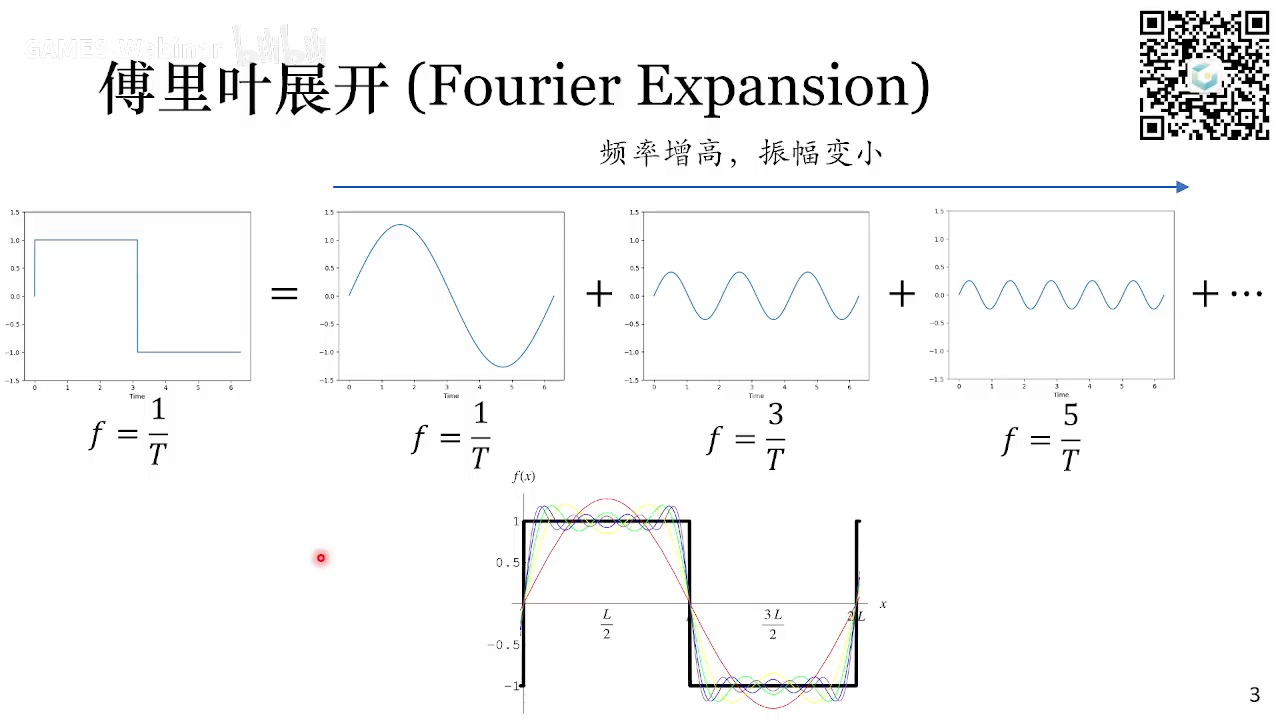
\includegraphics[width=0.92\textwidth]{figures/fig_01_fourier_square.jpg}
\caption{方波的傅里叶展开：频率增高、振幅变小的正弦函数之和\vtag}
\end{figure}
\srcnote{00:03:15--00:03:30}
\end{minipage}


把每个频率对应的振幅画出来，得到一张以频率为横轴的图，称为\textbf{频谱}（frequency spectrum），即振幅作为频率的函数。频谱是理解后面所有内容的关键概念：它告诉我们一个函数里“含有多少”各种频率的成分。维基百科上有一个很直观的动图：红色的信号沿着一个方向可以看成时间上的波形，换一个方向看，则是各个蓝色正弦分量的振幅排成的频谱。

\noindent\begin{minipage}{\textwidth}
\begin{figure}[H]
\centering
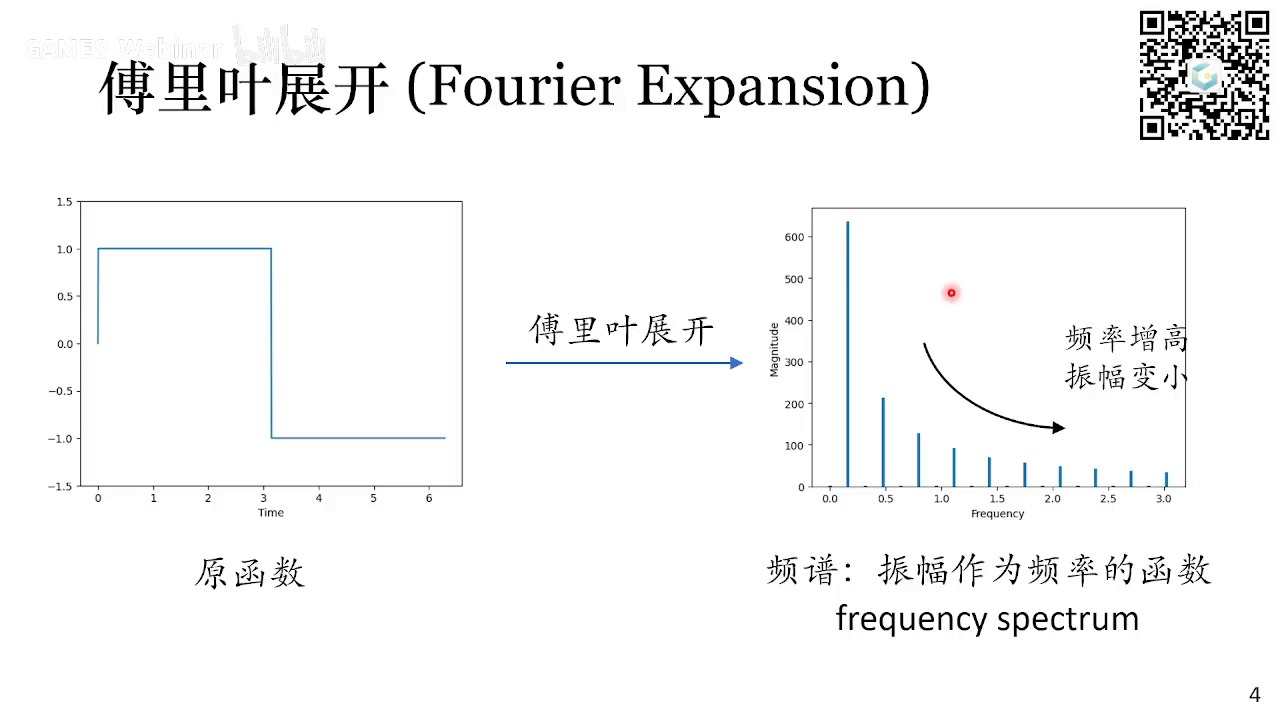
\includegraphics[width=0.92\textwidth]{figures/fig_02_spectrum.jpg}
\caption{傅里叶展开与频谱：原函数、各频率分量及其振幅\vtag}
\end{figure}
\srcnote{00:04:00--00:04:15}
\end{minipage}


\begin{knowledgebox}{方波为什么只有奇数倍频率}
课件中方波的分量频率是 $1/T,3/T,5/T,\dots$，没有偶数倍。讲义作者补充原因：以中心对称的方波为例，它满足 $f(t+T/2)=-f(t)$，即平移半个周期后正好取反。偶数倍频率的正弦平移半个周期后不变，与这种对称性矛盾，系数只能为零；奇数倍频率的正弦平移半个周期后恰好取反，与方波一致。具体计算可得第 $k$ 个奇数次谐波的振幅与 $1/k$ 成正比，所以频率越高振幅越小。
\end{knowledgebox}

\subsection{傅里叶级数的公式}

一般地，周期为 $T$ 的函数 $f(t)$ 可以展开为 $\cos\omega t,\sin\omega t,\cos2\omega t,\sin2\omega t,\dots$ 这样一系列三角函数的线性组合，其中 $\omega=2\pi/T$：
\[
f(t)=\frac{a_0}{2}+\sum_{n=1}^{\infty}\big(a_n\cos(n\omega t)+b_n\sin(n\omega t)\big),
\]
系数由积分给出：
\[
a_n=\frac2T\int_{-T/2}^{T/2}f(t)\cos(n\omega t)\,\mathrm dt,\qquad
b_n=\frac2T\int_{-T/2}^{T/2}f(t)\sin(n\omega t)\,\mathrm dt .
\]
课件用动画展示了把各项逐一加上去的过程：每多加一项，曲线就更接近原来的方波。

\noindent\begin{minipage}{\textwidth}
\begin{figure}[H]
\centering
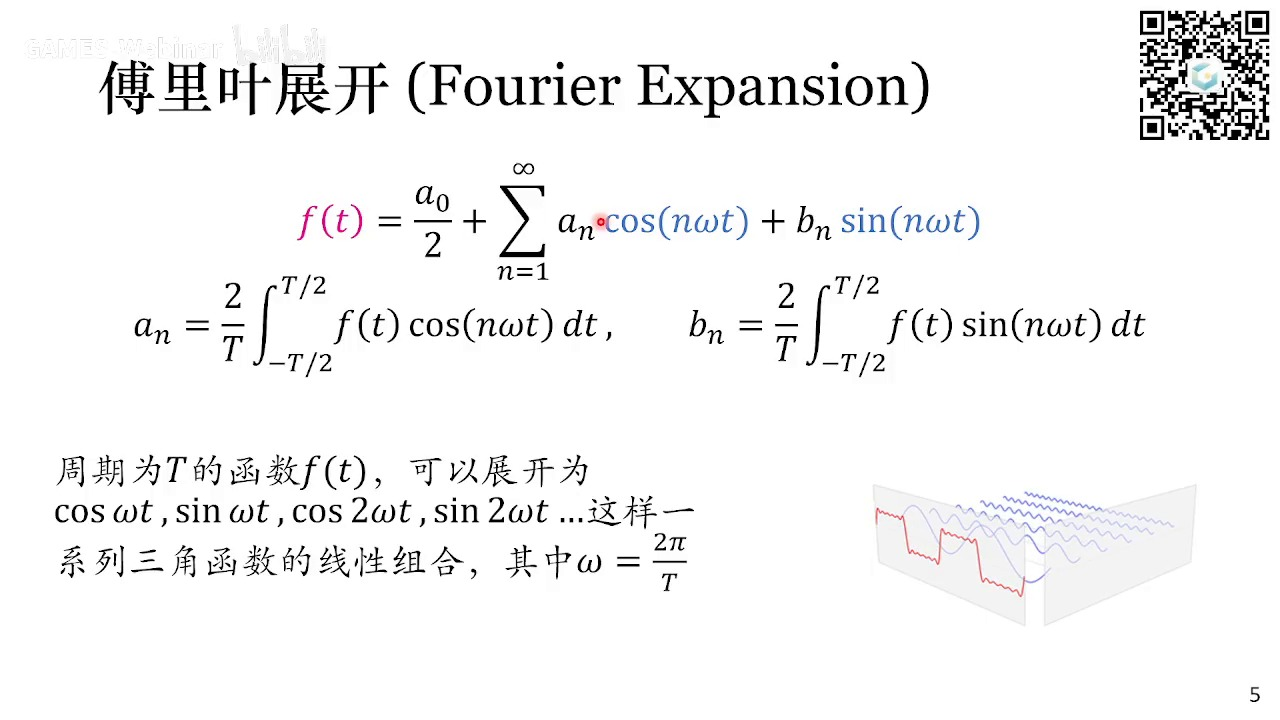
\includegraphics[width=0.92\textwidth]{figures/fig_03_fourier_series.jpg}
\caption{傅里叶级数：周期函数展开为三角函数的线性组合及其系数公式\vtag}
\end{figure}
\srcnote{00:04:30--00:04:45}
\end{minipage}


\noindent\begin{minipage}{\textwidth}
\begin{figure}[H]
\centering
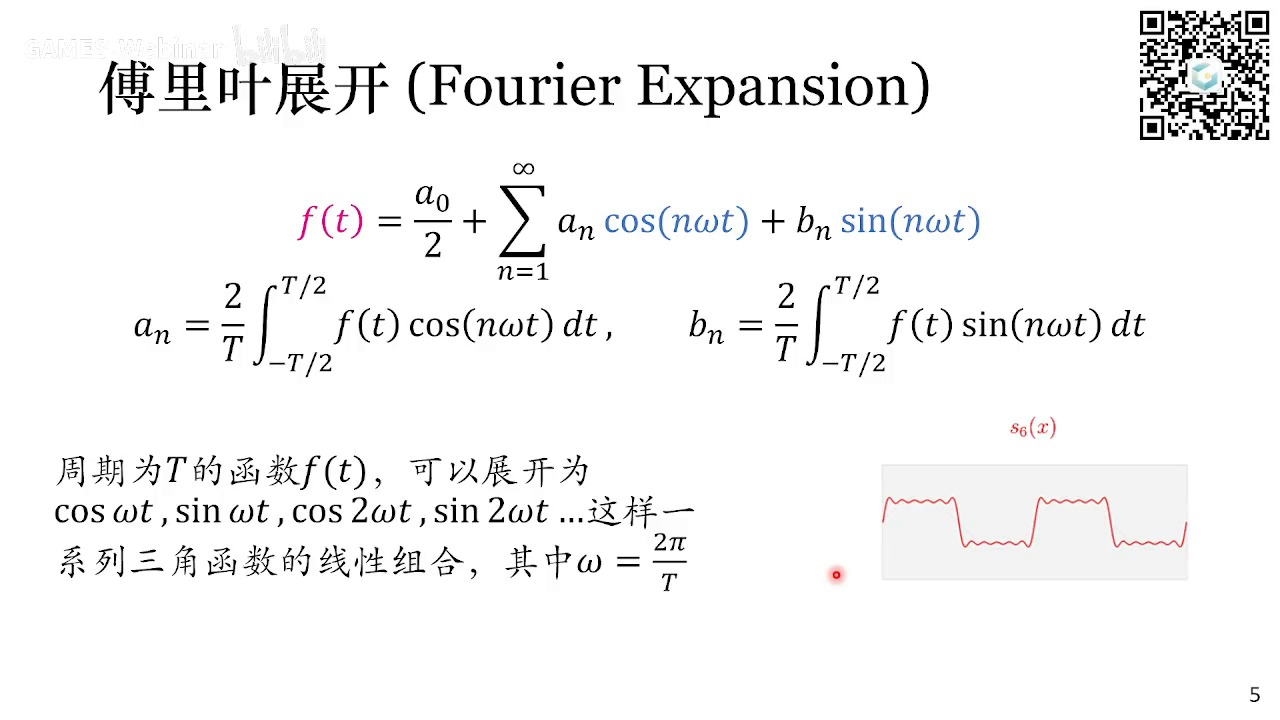
\includegraphics[width=0.92\textwidth]{figures/fig_04_fourier_partial.jpg}
\caption{逐项叠加的过程：项数越多，越接近原函数\vtag}
\end{figure}
\srcnote{00:05:30--00:05:45}
\end{minipage}


\subsection{指数形式}

利用欧拉公式 $e^{i\theta}=\cos\theta+i\sin\theta$，可以把余弦和正弦都写成只含 $e^{i\theta}$ 和 $e^{-i\theta}$ 的形式：
\[
\cos\theta=\frac12\big(e^{i\theta}+e^{-i\theta}\big),\qquad
\sin\theta=\frac1{2i}\big(e^{i\theta}-e^{-i\theta}\big).
\]
代入傅里叶级数，整理得到指数形式
\[
f(t)=\sum_{n=-\infty}^{\infty}c_ne^{in\omega t},\qquad
c_n=\frac1T\int_{-T/2}^{T/2}f(t)e^{-in\omega t}\,\mathrm dt .
\]
注意这里 $n$ 从负无穷取到正无穷，因为余弦和正弦里同时含有正、负指数。系数 $c_n$ 是复数，实部对应余弦，虚部对应正弦。讲者强调，这只是换了一种写法，反映的本质仍然是“把函数写成不同频率的三角函数之和”。

\noindent\begin{minipage}{\textwidth}
\begin{figure}[H]
\centering
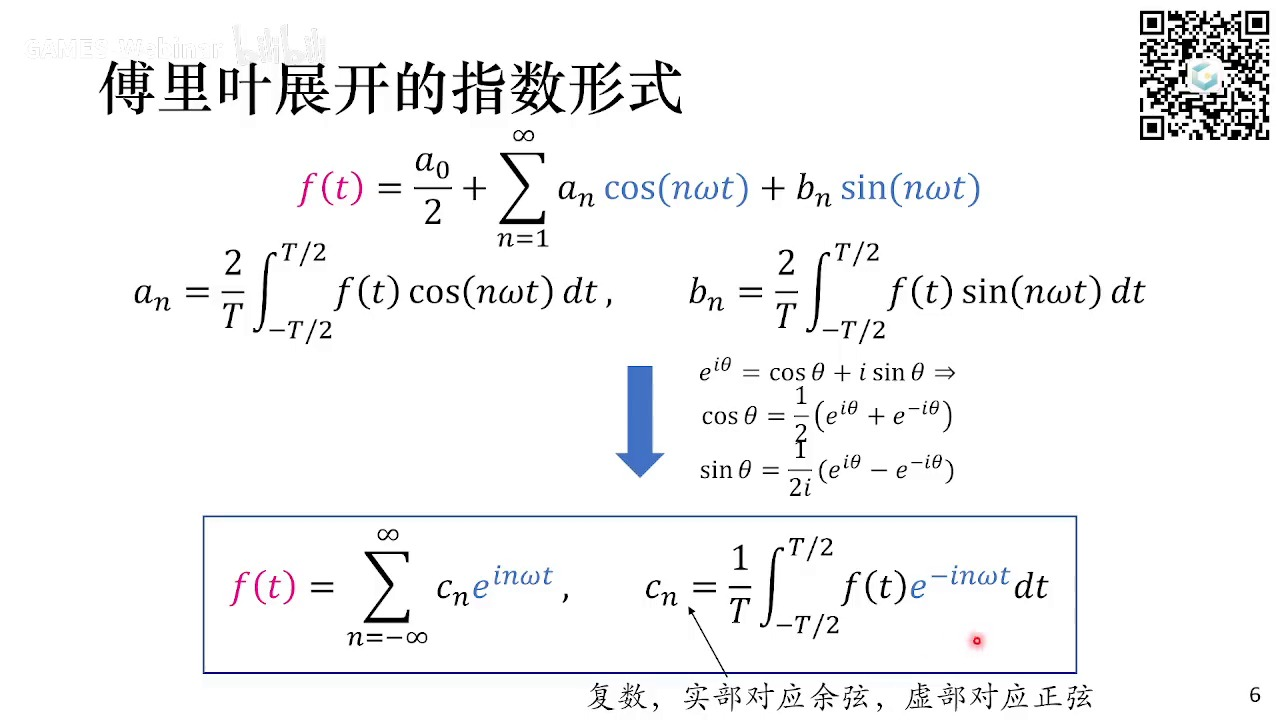
\includegraphics[width=0.92\textwidth]{figures/fig_05_exp_form.jpg}
\caption{傅里叶展开的指数形式：用欧拉公式把正弦余弦写成复指数\vtag}
\end{figure}
\srcnote{00:08:00--00:08:15}
\end{minipage}


\section{傅里叶变换}

\subsection{从周期函数到非周期函数}

傅里叶级数只适用于周期函数。对一般的非周期函数 $f(t)$，可以把它看成周期为无穷大的周期函数。此时 $\omega=2\pi/T$ 变为无穷小，相邻频率 $n\omega$ 之间的间隔趋于零，对 $n$ 的求和就变成对频率的积分：
\[
\lim_{\Delta x\to0}\sum_nf(n\Delta x)\,\Delta x=\int f(x)\,\mathrm dx .
\]
讲者解释，左边对 $n$ 的求和中，$n\omega$ 相乘出现，而 $\omega$ 正好扮演了 $\Delta x$ 的角色；当 $n$ 从负无穷取到正无穷时，这个求和等价于直接对函数积分。

\noindent\begin{minipage}{\textwidth}
\begin{figure}[H]
\centering
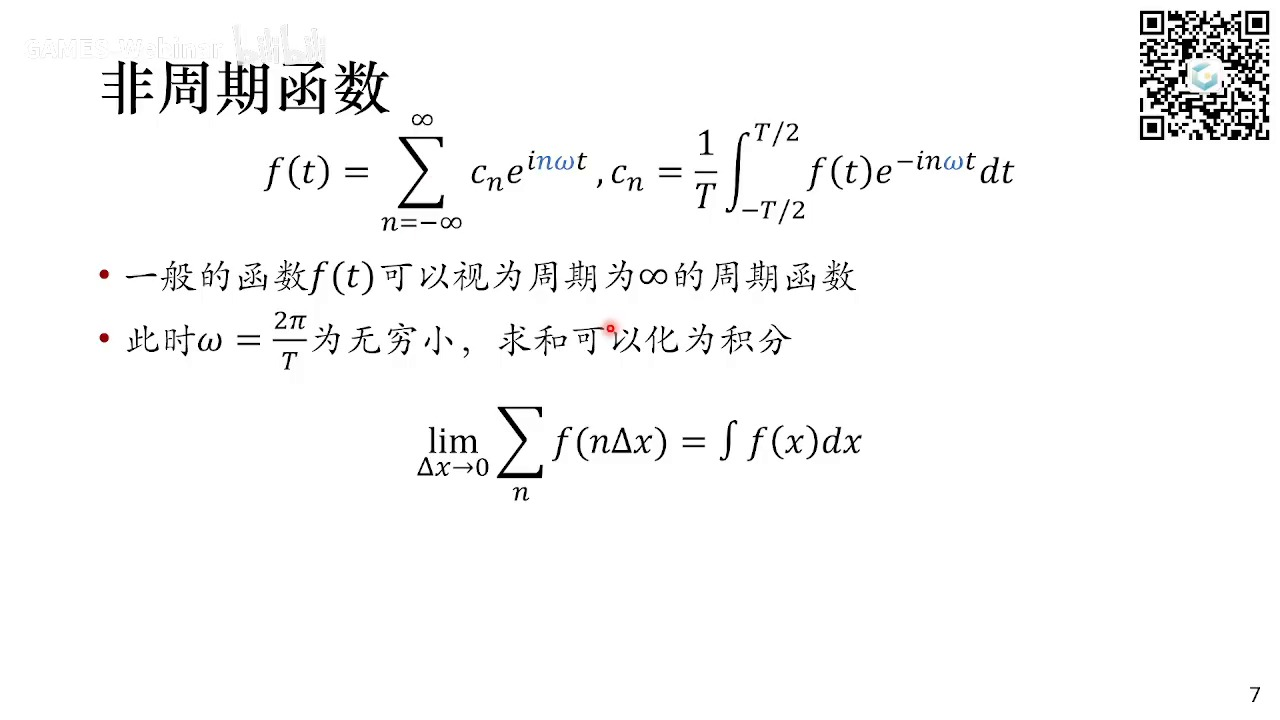
\includegraphics[width=0.92\textwidth]{figures/fig_06_nonperiodic.jpg}
\caption{非周期函数视为周期为无穷大的周期函数，求和化为积分\vtag}
\end{figure}
\srcnote{00:10:30--00:10:45}
\end{minipage}


取极限后，得到傅里叶变换对：
\[
f(t)=\int_{-\infty}^{\infty}F(\omega)e^{i\omega t}\,\mathrm d\omega,\qquad
F(\omega)=\frac{1}{2\pi}\int_{-\infty}^{\infty}f(t)e^{-i\omega t}\,\mathrm dt .
\]
$F(\omega)=\mathcal F(f)$ 称为 $f$ 的傅里叶变换，$f=\mathcal F^{-1}(F)$ 是逆变换。原来离散的系数 $c_n$ 变成了关于 $\omega$ 的连续函数 $F(\omega)$。讲者提醒，课件中有一处 $\omega$ 的上下标在推导时没写清楚，这里的 $\omega$ 已经是连续的频率变量。

\noindent\begin{minipage}{\textwidth}
\begin{figure}[H]
\centering
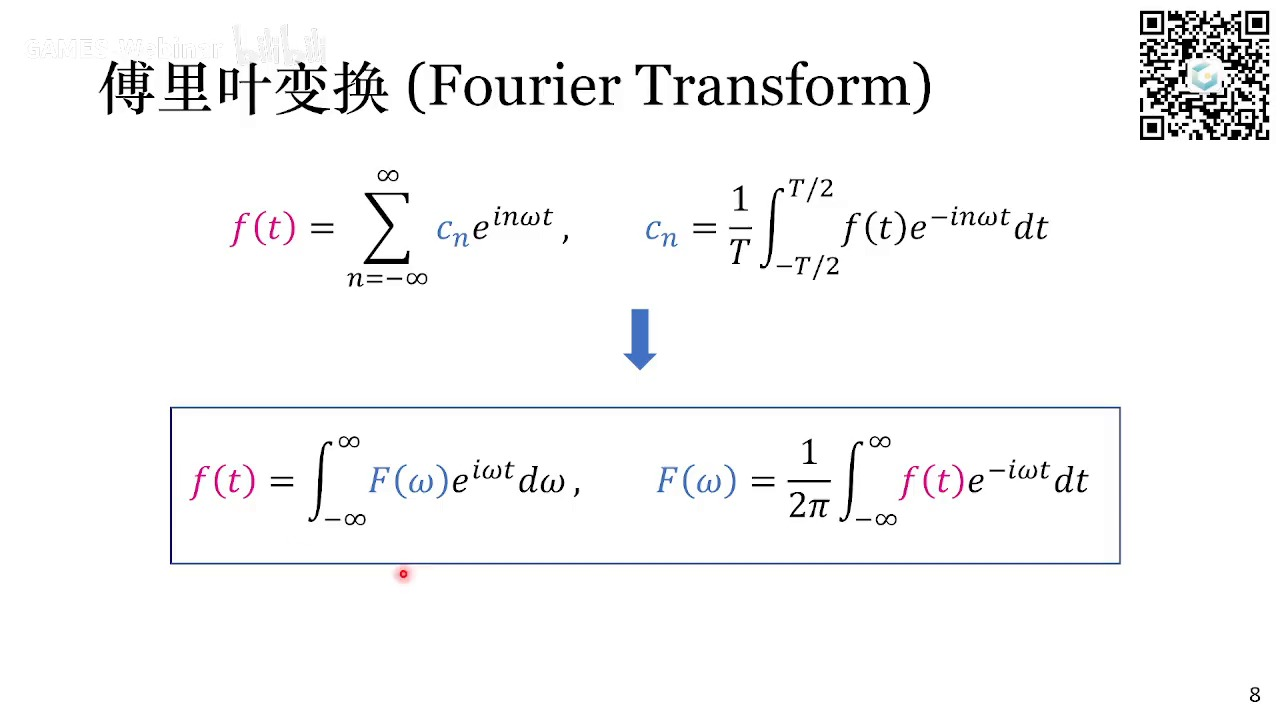
\includegraphics[width=0.92\textwidth]{figures/fig_07_fourier_transform.jpg}
\caption{傅里叶变换对：$f(t)$ 与 $F(\omega)$\vtag}
\end{figure}
\srcnote{00:11:45--00:12:00}
\end{minipage}


课件中的例子是一个非周期函数：在 $[-T/2,T/2]$ 之间取常数，其他地方都为零，即一个矩形脉冲。它的傅里叶变换是连续的，中间是一个高峰，两侧是逐渐衰减的振荡。周期函数的频谱是一根根离散的谱线，非周期函数的频谱则是连续的。

\noindent\begin{minipage}{\textwidth}
\begin{figure}[H]
\centering
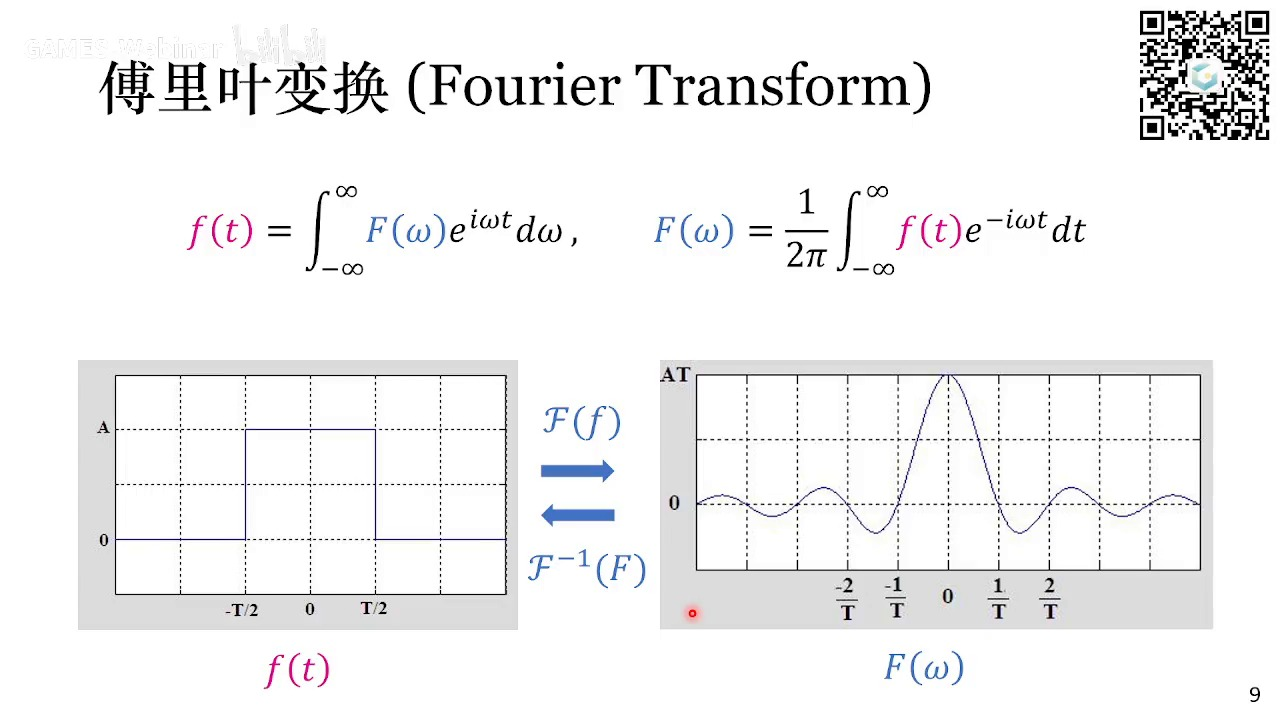
\includegraphics[width=0.92\textwidth]{figures/fig_08_rect_transform.jpg}
\caption{矩形脉冲的傅里叶变换：非周期函数的频谱是连续的\vtag}
\end{figure}
\srcnote{00:13:15--00:13:30}
\end{minipage}


\begin{warningbox}{$2\pi$ 放在哪里有不同约定}
讲义作者提醒：傅里叶变换的归一化系数有多种约定。课件把 $\frac1{2\pi}$ 放在正变换上；也有教材把它放在逆变换上，或者两边各放 $\frac1{\sqrt{2\pi}}$，还有用频率 $\xi$ 代替角频率 $\omega$、写成 $e^{-2\pi i\xi t}$ 从而完全不出现系数的写法。不同约定下，卷积定理、梳状函数的变换等公式会相差常数因子。查阅资料或调用 FFT 库时，一定要先确认它用的是哪种约定。
\end{warningbox}

\subsection{用线性代数理解傅里叶变换}

讲者说，他希望今天能帮助大家理解傅里叶变换的\emph{本质}。傅里叶变换为我们提供了另外一个视角来理解函数（信号），称为\textbf{频域}（frequency domain）。用线性代数来理解：在三维空间中，向量可以写成 $\mathbf x=\sum_ia_i\mathbf e_i$，其中 $\mathbf e_i$ 是基向量，$a_i$ 是向量在各个轴上的分量。傅里叶变换做的是同一件事，只不过现在的“向量”都是函数：
\[
f(t)=\int_{-\infty}^{\infty}F(\omega)\,e^{i\omega t}\,\mathrm d\omega\quad\longleftrightarrow\quad\mathbf x=\sum_ia_i\mathbf e_i .
\]
$\{e^{i\omega t}\mid\omega\in\mathbb R\}$ 构成了一组基，它有无穷多个“向量”；$F(\omega)$ 就是对应每个基的组合系数。唯一的不同是，三维空间里基是有限个，所以做求和；这里基有无穷多个且连续，所以做积分。

那么问题来了：$f(t)$ 原来的基是什么？我们平时写 $f(t)$ 的时候，又是在哪组基下展开的？

\noindent\begin{minipage}{\textwidth}
\begin{figure}[H]
\centering
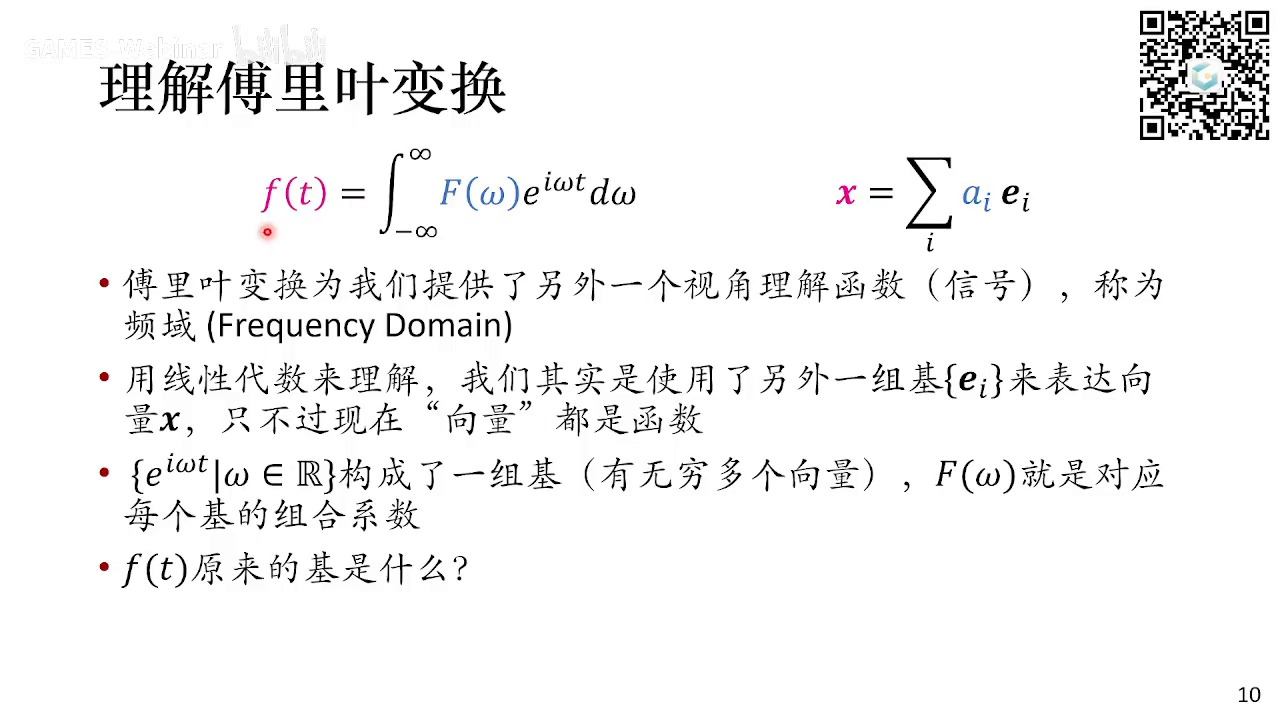
\includegraphics[width=0.92\textwidth]{figures/fig_09_understand_ft.jpg}
\caption{理解傅里叶变换：$\{e^{i\omega t}\}$ 是一组基，$F(\omega)$ 是组合系数\vtag}
\end{figure}
\srcnote{00:20:45--00:21:00}
\end{minipage}


\subsection{Delta 函数}

为了回答这个问题，需要引入 \textbf{Delta 函数}，也叫狄拉克 $\delta$ 函数。它是一个很奇怪的存在：
\[
\delta(t)=\begin{cases}\infty,&t=0\\0,&t\neq0\end{cases},\qquad \int_{-\infty}^{\infty}\delta(t)\,\mathrm dt=1 .
\]
它在零点处是一个无限高的“尖”，其他地方都是零，但积分结果为一。$\delta(t-a)$ 就是在 $a$ 处的一个尖。可以把它想象成一族越来越窄、越来越高、面积始终为一的高斯函数的极限。

\begin{warningbox}{Delta 函数不是普通函数}
讲义作者提醒：按普通函数的意义，一个只在一点非零的函数积分应为零，所以 $\delta$ 并不是真正的函数，而是一种“广义函数”（分布），只有放在积分里、与别的函数相乘后才有确定的意义。上面的写法是物理和工程中通行的直观记法，用来推导结论没有问题，但不要对 $\delta(t)$ 本身做逐点运算，比如求 $\delta(t)^2$。
\end{warningbox}

\noindent\begin{minipage}{\textwidth}
\begin{figure}[H]
\centering
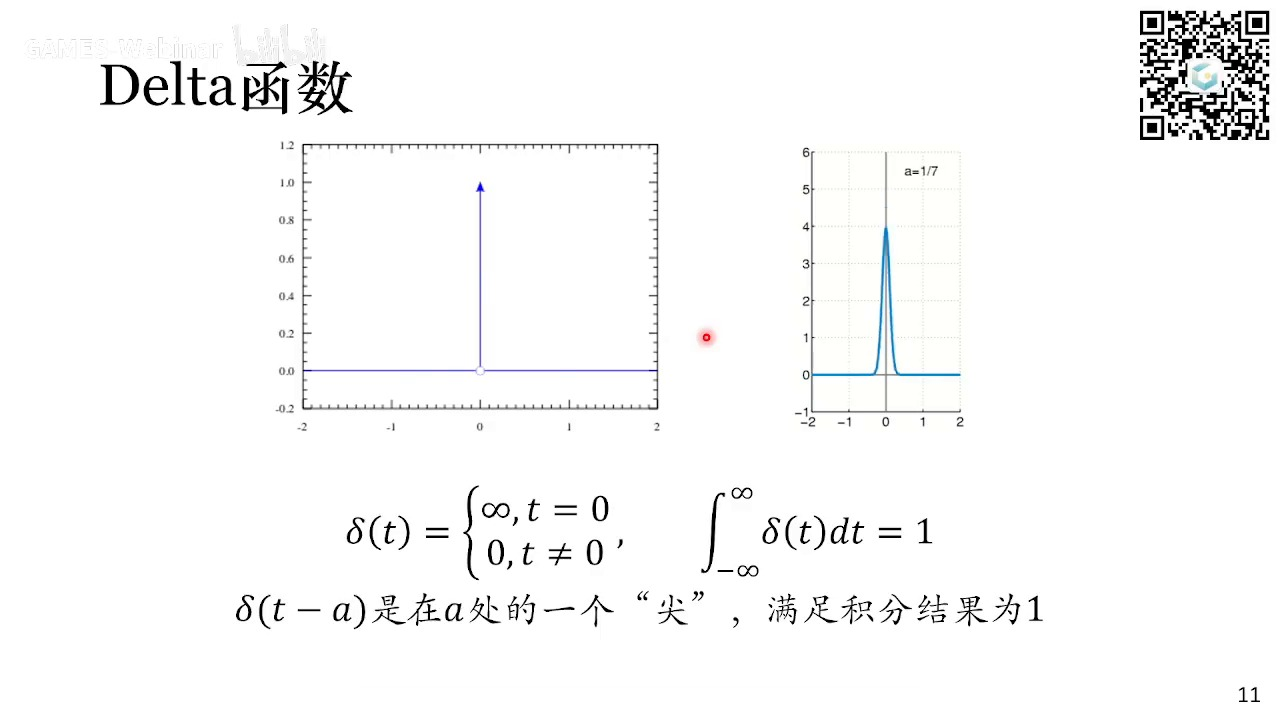
\includegraphics[width=0.92\textwidth]{figures/fig_10_delta.jpg}
\caption{Delta 函数：在 $a$ 处的一个“尖”，积分为一\vtag}
\end{figure}
\srcnote{00:22:45--00:23:00}
\end{minipage}


Delta 函数最重要的性质是下面的积分恒等式。对任意函数 $f$，考察积分 $\int f(a)\delta(t-a)\,\mathrm da$。当 $a\neq t$ 时 $\delta(t-a)=0$，被积函数为零，所以只需考虑 $t$ 的一个小邻域 $(t-\varepsilon,t+\varepsilon)$；在这个邻域内 $f(a)$ 近似等于 $f(t)$，可以提到积分外面：
\[
\int_{-\infty}^{\infty}f(a)\delta(t-a)\,\mathrm da=\lim_{\varepsilon\to0}\int_{t-\varepsilon}^{t+\varepsilon}f(a)\delta(t-a)\,\mathrm da=f(t)\lim_{\varepsilon\to0}\int_{t-\varepsilon}^{t+\varepsilon}\delta(t-a)\,\mathrm da=f(t).
\]

\noindent\begin{minipage}{\textwidth}
\begin{figure}[H]
\centering
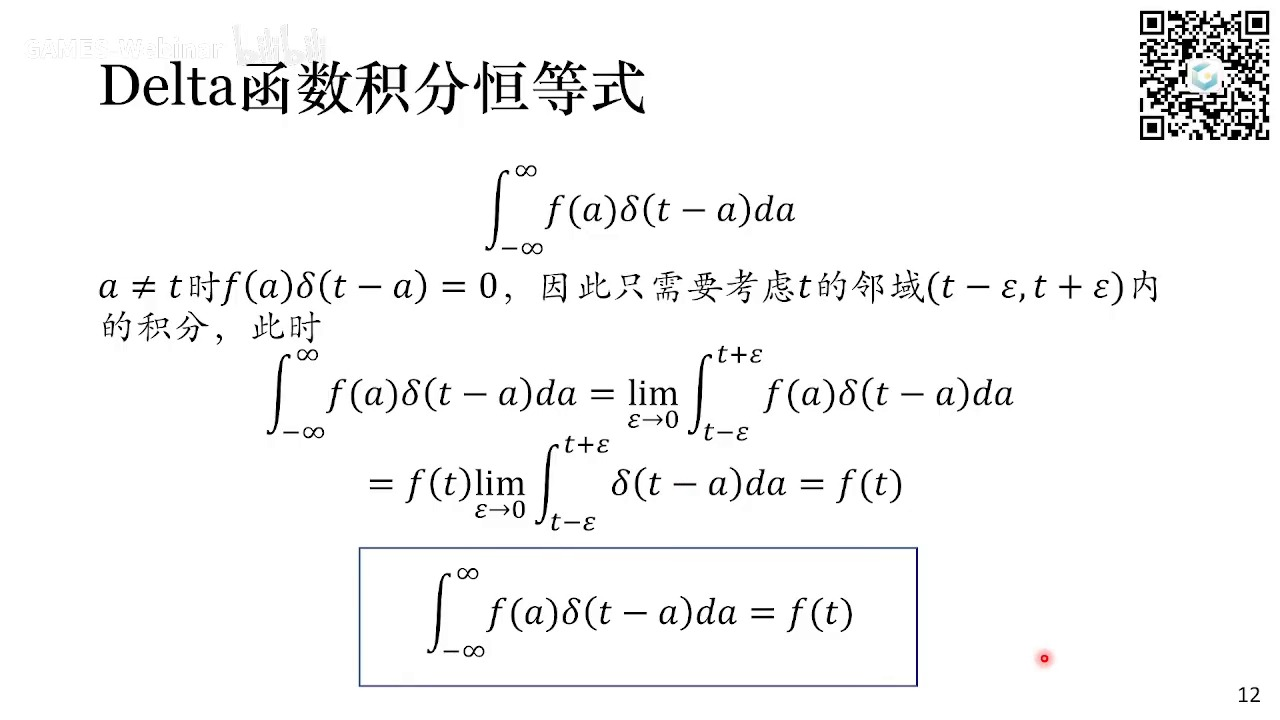
\includegraphics[width=0.92\textwidth]{figures/fig_11_delta_identity.jpg}
\caption{Delta 函数的积分恒等式：$\int f(a)\delta(t-a)\,\mathrm da=f(t)$\vtag}
\end{figure}
\srcnote{00:24:45--00:25:00}
\end{minipage}


\subsection{函数原来的基}

把这个恒等式仔细观察一下：
\[
f(t)=\int_{-\infty}^{\infty}f(a)\,\delta(t-a)\,\mathrm da\quad\longleftrightarrow\quad\mathbf x=\sum_ia_i\mathbf e_i .
\]
在线性代数的视角下，$\{\delta(t-a)\mid a\in\mathbb R\}$ 是一组基，每一个基向量 $\delta(t-a)$ 是关于 $t$ 的函数，而 $f(a)$ 是对应基向量 $\delta(t-a)$ 的系数。需要注意的是，这里的系数 $f(a)$ 其实就是函数 $f(t)$ 本身。

讲者用三维空间类比：一个向量 $\mathbf v$ 可以表示为三维坐标 $(v_x,v_y,v_z)$；默认情况下，我们直接用 $(v_x,v_y,v_z)$ 指代向量 $\mathbf v$ 本身，而不强调这是在三维笛卡尔坐标系下的分解。对应到函数的线性空间，当我们把函数写成 $f(t)$ 的时候，其实也默认了以 $\{\delta(t-a)\}$ 为基底进行展开，直接给出了展开的系数。

\begin{importantbox}{理解时域表示的关键}
我们平时说“一个函数 $f(t)$”，其实已经隐含选定了一组基：每个时刻 $a$ 上的一个尖 $\delta(t-a)$。$f$ 在 $a$ 处的取值，就是这组基下的第 $a$ 个坐标。一旦接受这一点，傅里叶变换就不再神秘：它只是把同一个“向量”换到另一组基 $\{e^{i\omega t}\}$ 下重新读坐标，读出来的坐标就是 $F(\omega)$。
\end{importantbox}

\noindent\begin{minipage}{\textwidth}
\begin{figure}[H]
\centering
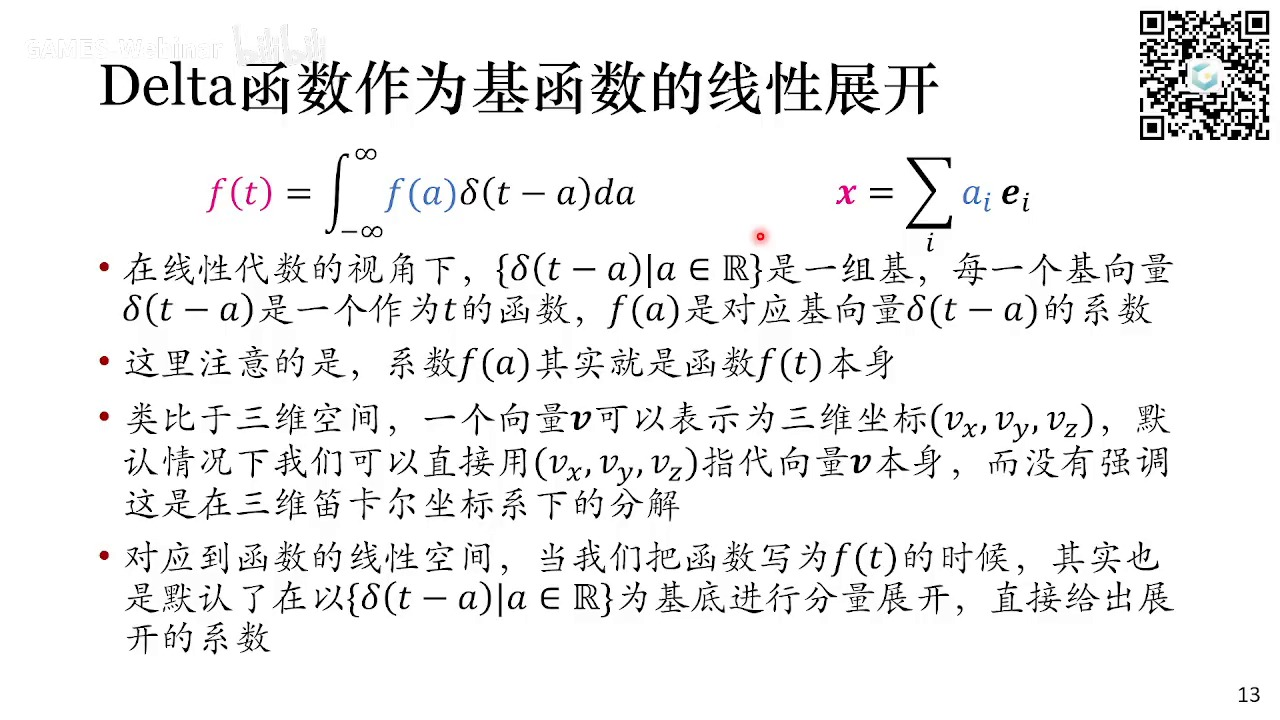
\includegraphics[width=0.92\textwidth]{figures/fig_12_delta_basis.jpg}
\caption{Delta 函数作为基函数：写出 $f(t)$ 就是在 Delta 基下给出系数\vtag}
\end{figure}
\srcnote{00:28:45--00:29:00}
\end{minipage}


\subsection{时域与频域}

于是时域和频域的关系就非常清楚了：
\begin{itemize}
\item \textbf{时域}：$f(t)=\int f(a)\delta(t-a)\,\mathrm da$，基函数是 Delta 函数 $\delta(t-a)$，系数是 $f(a)$；
\item \textbf{频域}：$f(t)=\int F(\omega)e^{i\omega t}\,\mathrm d\omega$，基函数是三角函数 $e^{i\omega t}$，系数是 $F(\omega)$。
\end{itemize}
傅里叶变换做的事情非常直接：对同一个函数，换了一组基函数来做展开，拿到新的展开系数，用它来代替原来的系数。这就是本讲第一句话“傅里叶变换是从时域基底换到频域基底的线性变换”的含义。讲者说，因为时间有限，今天只能做这种比较抽象、不涉及严格证明的描述，但这是他今天最想传达的观点。

\noindent\begin{minipage}{\textwidth}
\begin{figure}[H]
\centering
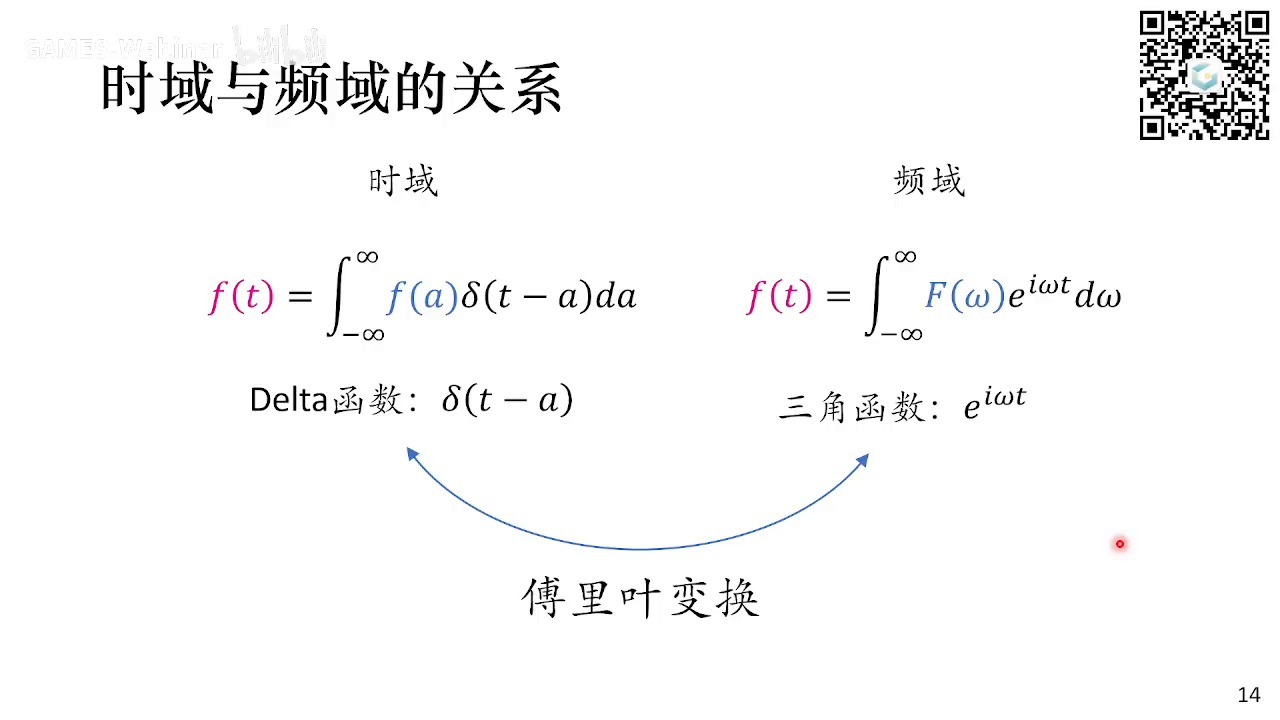
\includegraphics[width=0.92\textwidth]{figures/fig_13_time_freq.jpg}
\caption{时域与频域的关系：Delta 基与三角函数基之间的基变换\vtag}
\end{figure}
\srcnote{00:31:15--00:31:30}
\end{minipage}


\begin{knowledgebox}{和 SVD、PCA 的类比}
讲义作者补充：上一讲的 SVD 和 PCA 也是在“换基”：PCA 用协方差矩阵的特征向量作为新基，按方差从大到小排列，截断后得到低维表示。傅里叶变换用的是三角函数基，按频率排列。二者都把数据在一组正交基下重新展开，然后只保留重要的系数，所以下面的图像压缩与 SVD 压缩在思想上完全一致。区别在于傅里叶基是固定的、与数据无关，而 PCA 的基是从数据中学出来的。
\end{knowledgebox}

\section{离散傅里叶变换与图像应用}

\subsection{离散傅里叶变换与 FFT}

计算机中处理的都是离散信号。把连续的傅里叶变换离散化，得到离散傅里叶变换（DFT）。对 $N$ 个采样值 $x[p]$：
\[
X[k]=\sum_px[p]\,e^{-i\frac{2\pi}{N}kp},\qquad
x[p]=\frac1N\sum_kX[k]\,e^{i\frac{2\pi}{N}kp}.
\]
原本连续的正弦函数，都变成了离散的、按分辨率采样的正弦序列。直接计算 DFT 需要 $O(N^2)$ 次运算。快速傅里叶变换（FFT）利用分治、递归的思想，把长度为 $N$ 的变换拆成两个长度为 $N/2$ 的变换，复杂度降到 $O(N\log N)$。它是应用最广泛的算法之一。

\noindent\begin{minipage}{\textwidth}
\begin{figure}[H]
\centering
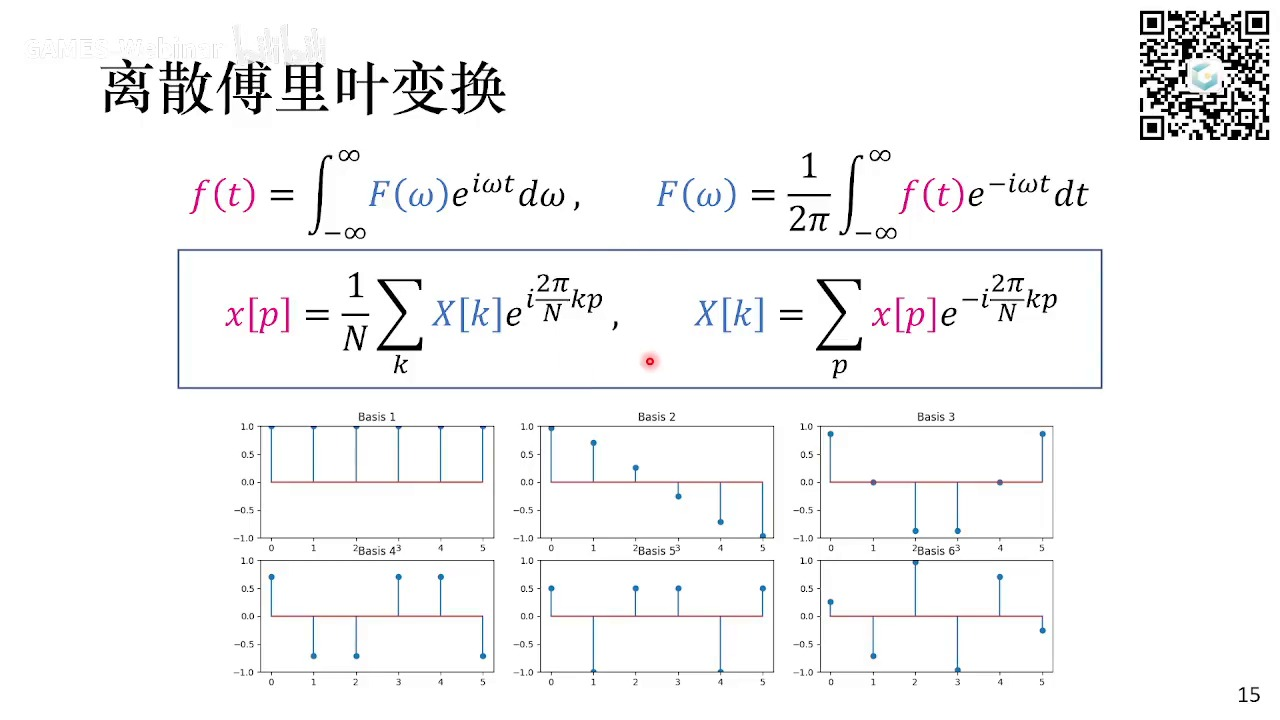
\includegraphics[width=0.92\textwidth]{figures/fig_14_dft.jpg}
\caption{离散傅里叶变换：连续变换的离散对应\vtag}
\end{figure}
\srcnote{00:32:45--00:33:00}
\end{minipage}


\noindent\begin{minipage}{\textwidth}
\begin{figure}[H]
\centering
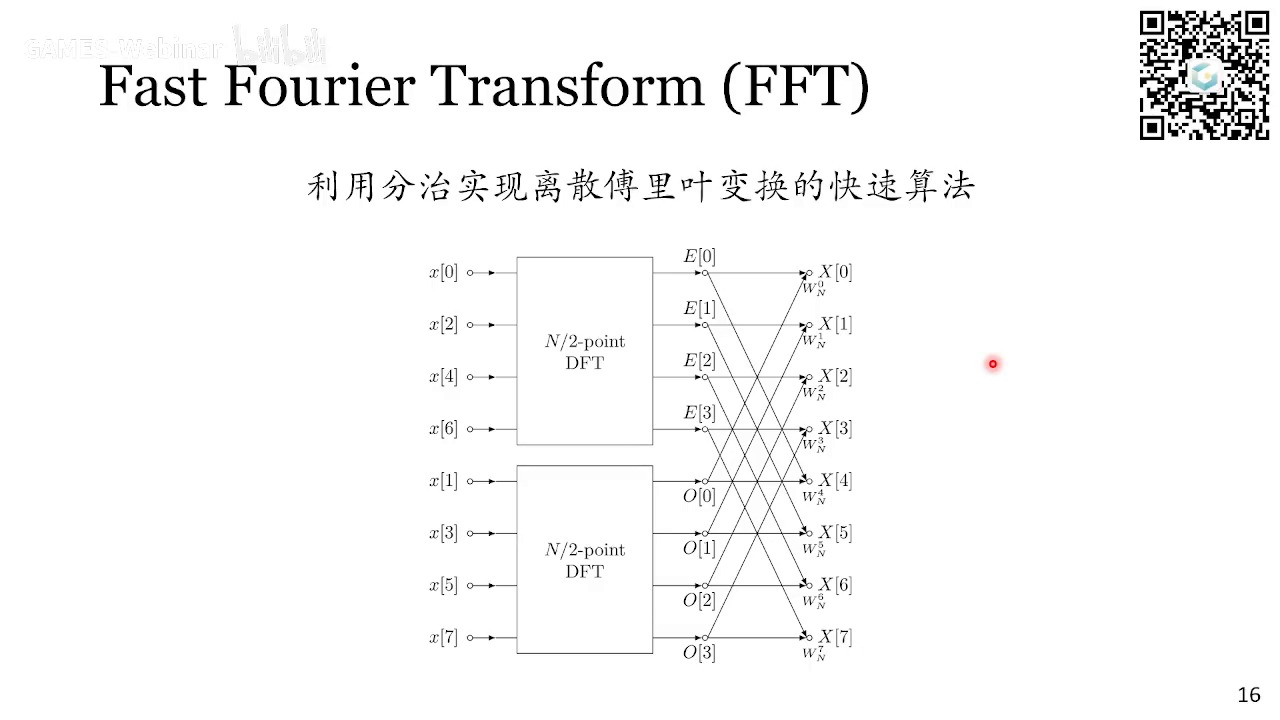
\includegraphics[width=0.92\textwidth]{figures/fig_15_fft.jpg}
\caption{快速傅里叶变换：利用分治实现 DFT 的快速算法\vtag}
\end{figure}
\srcnote{00:33:45--00:34:00}
\end{minipage}


\subsection{图像去噪与压缩}

傅里叶变换的经典应用是图像处理。图片可以看成二维函数，沿 $x$、$y$ 两个方向分别做傅里叶变换，得到二维频谱，横纵坐标为 $(\omega_x,\omega_y)$。频谱中心对应低频，离中心越远频率越高。

\noindent\begin{minipage}{\textwidth}
\begin{figure}[H]
\centering
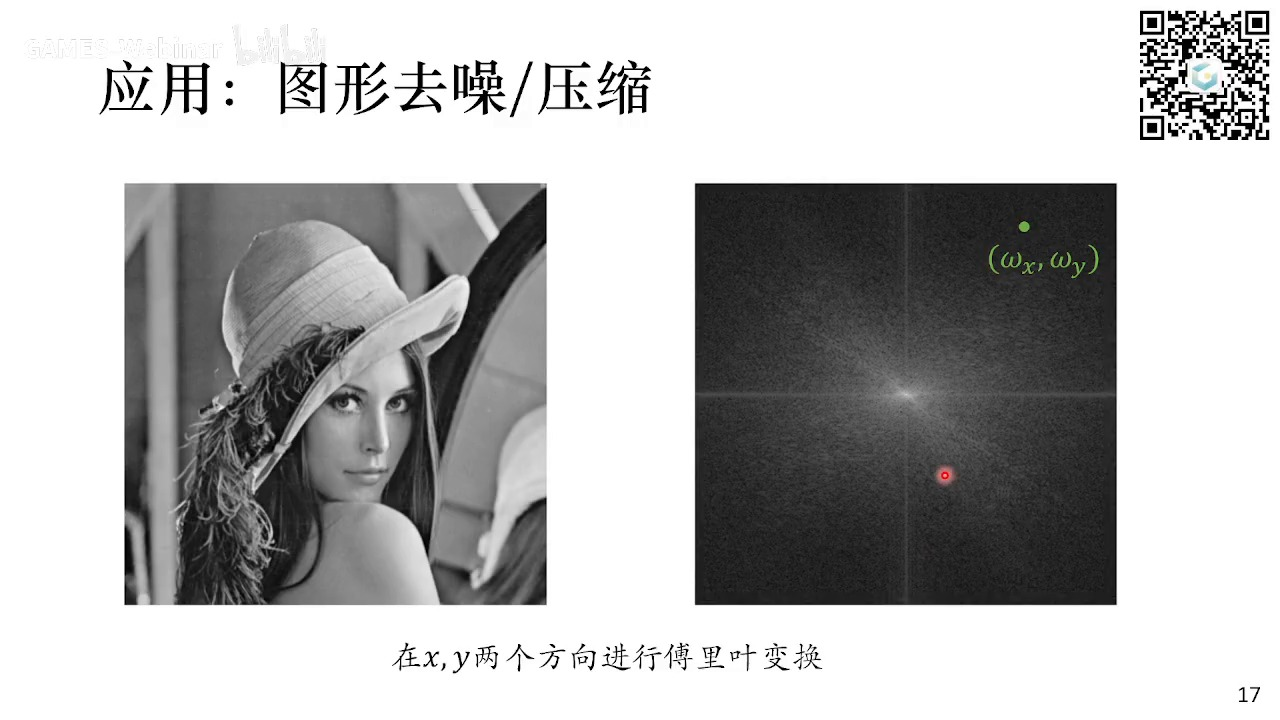
\includegraphics[width=0.92\textwidth]{figures/fig_16_image_ft.jpg}
\caption{图像的二维傅里叶变换：中心为低频，向外为高频\vtag}
\end{figure}
\srcnote{00:34:45--00:35:00}
\end{minipage}


\textbf{低通滤波}：把频谱中离中心远的高频部分直接裁掉，只保留中心附近的部分，再做逆傅里叶变换，得到的图片会变模糊，因为高频信息代表的细节和边缘丢失了；保留的范围越小，图片越模糊。反过来看，只保留低频信息就能大致还原图片，这就实现了图像压缩。讲者指出，这与上一讲 SVD 压缩的思想是类似的。

\noindent\begin{minipage}{\textwidth}
\begin{figure}[H]
\centering
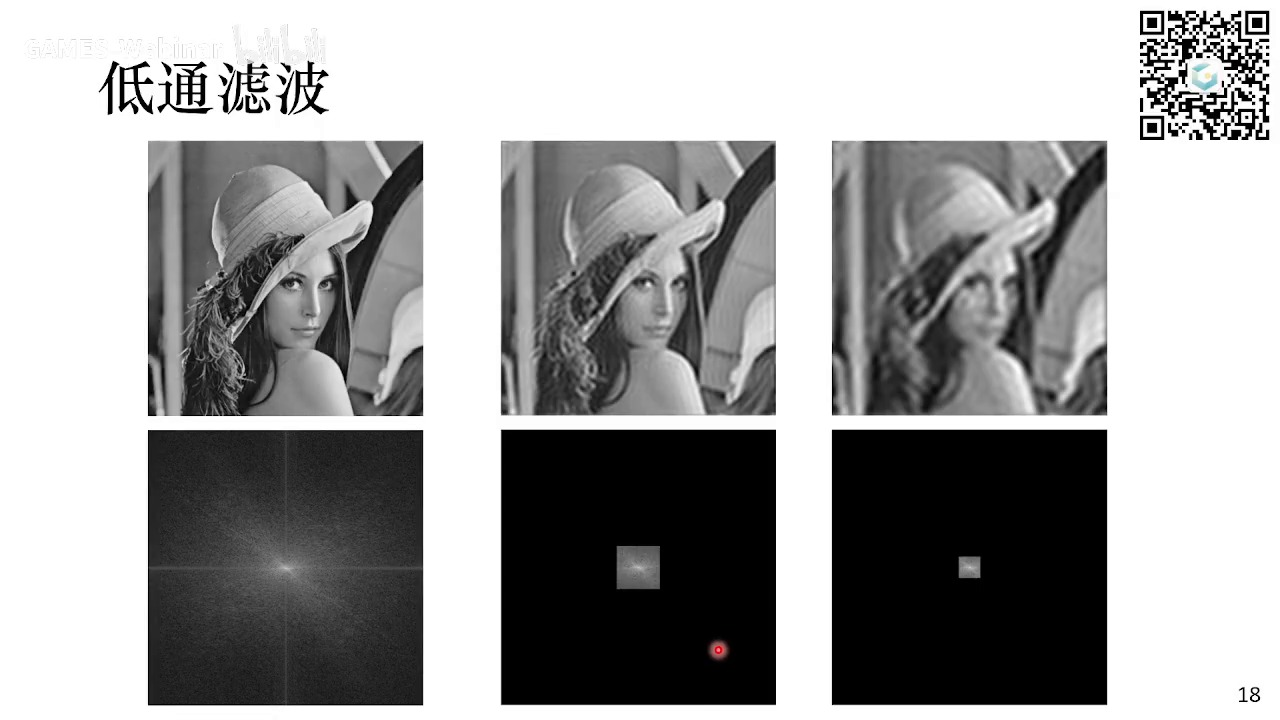
\includegraphics[width=0.92\textwidth]{figures/fig_17_lowpass.jpg}
\caption{低通滤波：只保留频谱中心的低频部分，图片变模糊\vtag}
\end{figure}
\srcnote{00:37:00--00:37:15}
\end{minipage}


\textbf{边缘提取}：反之，如果把中间的低频信息全都挖掉，只保留高频信息，逆变换后得到的就是图片的边缘和细节。

\noindent\begin{minipage}{\textwidth}
\begin{figure}[H]
\centering
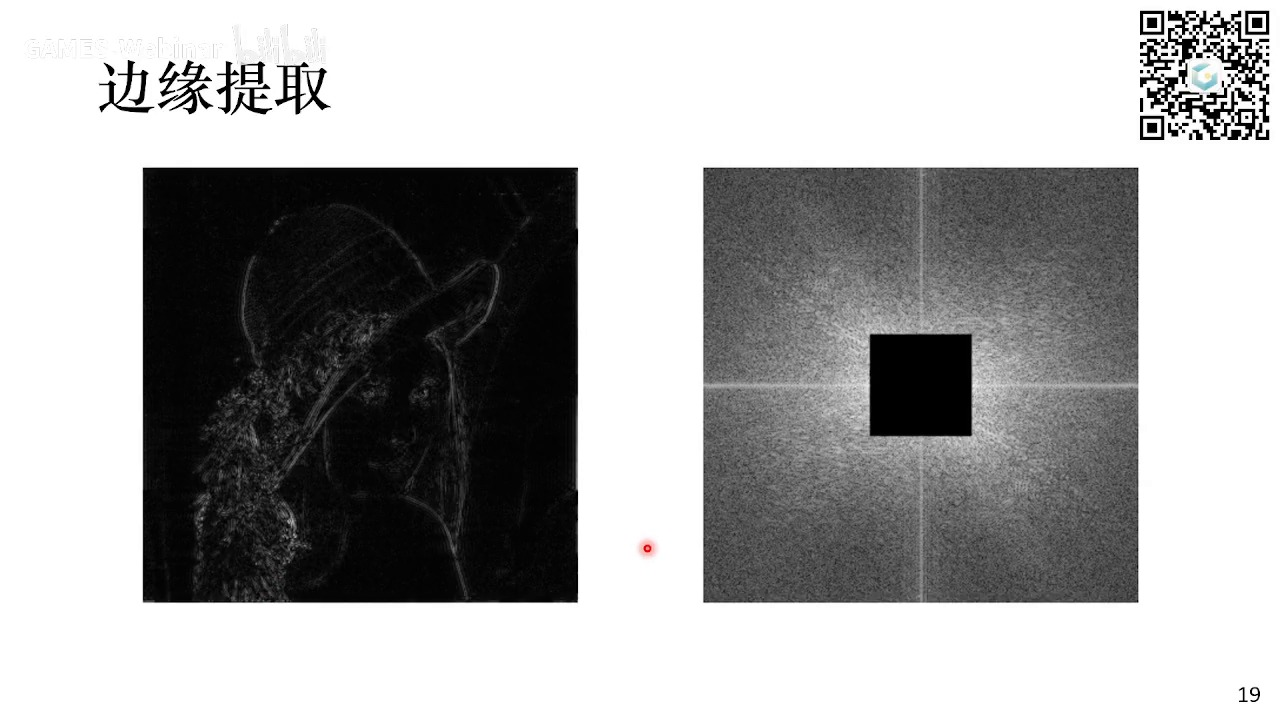
\includegraphics[width=0.92\textwidth]{figures/fig_18_edge.jpg}
\caption{边缘提取：挖掉低频只保留高频，得到图像的边缘\vtag}
\end{figure}
\srcnote{00:37:45--00:38:00}
\end{minipage}


\begin{practicebox}{动手做频域滤波}
用任意语言读入一张灰度图，调用二维 FFT 并把零频移到中心；分别用半径为 10、30、80 像素的圆形掩码保留低频，逆变换后观察图像模糊程度；再用相反的掩码只保留高频，观察提取出的边缘。最后比较：保留同样数量的系数时，傅里叶截断和上一讲的 SVD 截断，哪一个重建效果更好？
\end{practicebox}

\section{卷积}

\subsection{图像卷积}

卷积（convolution）是与傅里叶变换密切相关的概念。GAMES101 中介绍过图像卷积：取一个卷积核，比如 $3\times3$、每个元素为 $\frac19$ 的平均核，把它放在图片上，与对应位置的像素相乘再相加，得到的值放到新图片的对应位置；然后把卷积核在图片上不断滑动，重复这个操作。用平均核卷积后，图片变得平滑。

\noindent\begin{minipage}{\textwidth}
\begin{figure}[H]
\centering
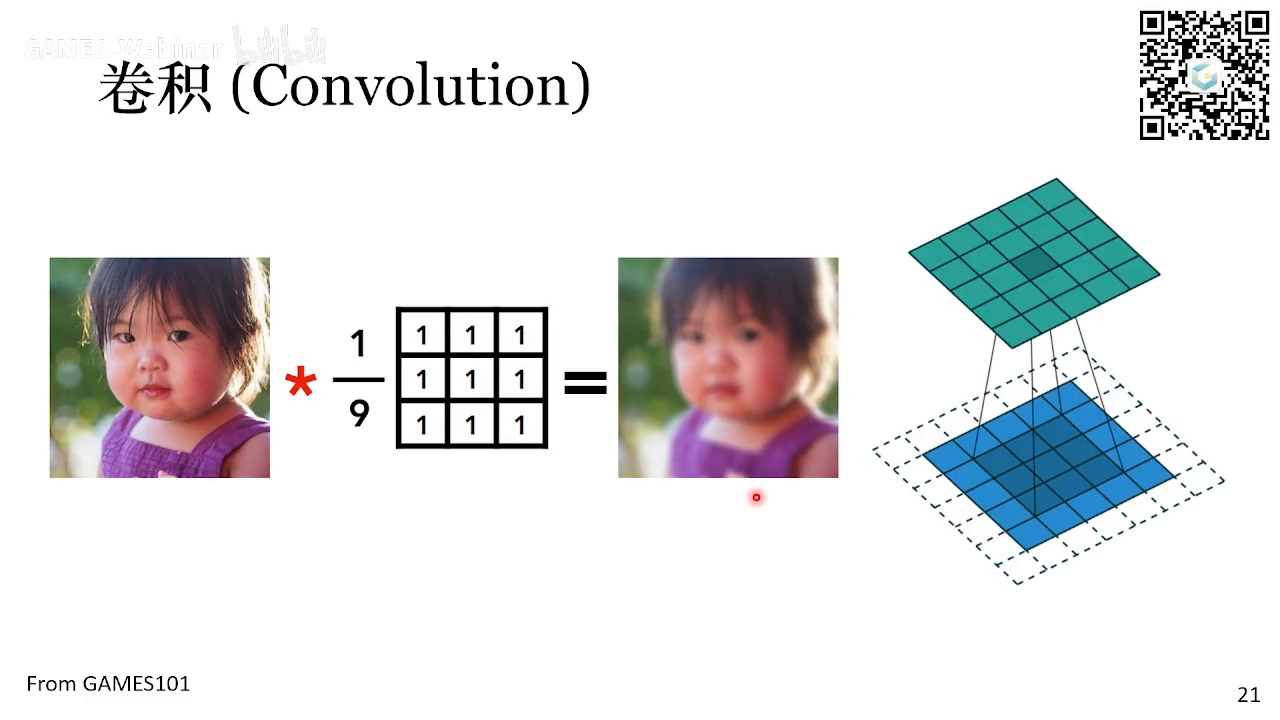
\includegraphics[width=0.92\textwidth]{figures/fig_19_conv_image.jpg}
\caption{图像卷积：平均核在图片上滑动，相乘相加，使图片平滑\vtag}
\end{figure}
\srcnote{00:39:15--00:39:30}
\end{minipage}


\subsection{卷积的定义}

连续函数的卷积定义为
\[
(f*g)(t)=\int f(\tau)\,g(t-\tau)\,\mathrm d\tau .
\]
这是关于 $\tau$ 的积分，$t$ 是给定的常数，结果是 $f*g$ 在 $t$ 处的值。$g(t-\tau)$ 作为 $\tau$ 的函数，是 $g(\tau)$ 以 $t/2$ 为中点做的镜像。随着 $t$ 从零开始增大，镜像后的 $g(t-\tau)$ 不断往右平移，与 $f(\tau)$ 的重合部分不断变化，把重合部分乘起来积分，就得到每个 $t$ 处的卷积值。所以卷积就是：把卷积核做镜像，在信号上不断滑动，计算它们重合部分的乘积之和。

\noindent\begin{minipage}{\textwidth}
\begin{figure}[H]
\centering
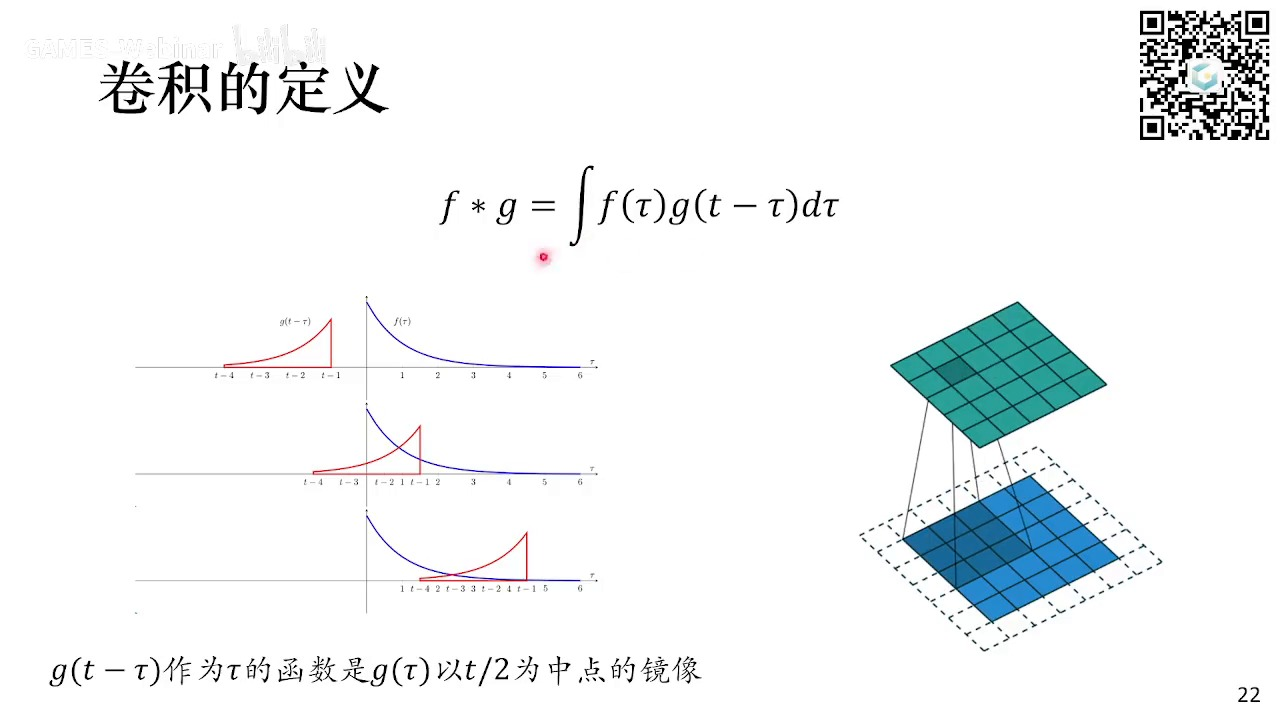
\includegraphics[width=0.92\textwidth]{figures/fig_20_conv_def.jpg}
\caption{卷积的定义：$g(t-\tau)$ 是 $g(\tau)$ 的镜像，随 $t$ 平移\vtag}
\end{figure}
\srcnote{00:39:30--00:39:45}
\end{minipage}


\noindent\begin{minipage}{\textwidth}
\begin{figure}[H]
\centering
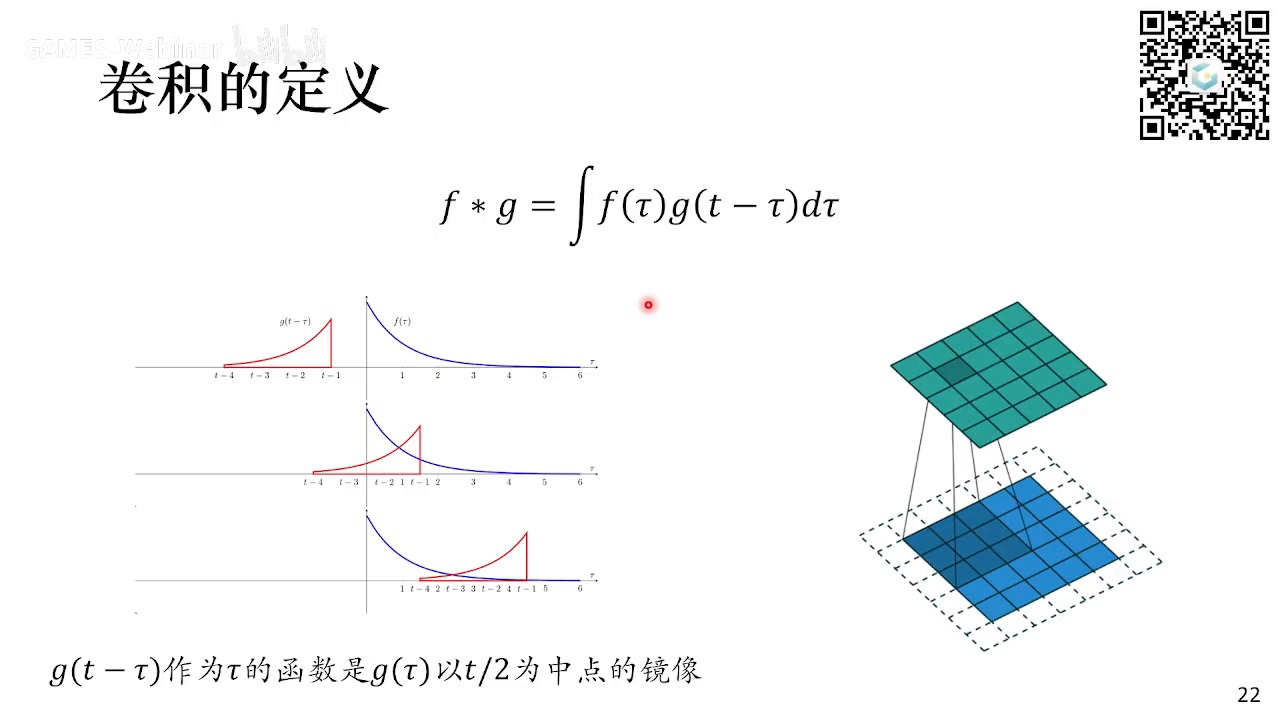
\includegraphics[width=0.92\textwidth]{figures/fig_21_conv_slide.jpg}
\caption{卷积的滑动过程：镜像后的核不断平移，与信号重合部分相乘积分\vtag}
\end{figure}
\srcnote{00:42:00--00:42:15}
\end{minipage}


\begin{warningbox}{卷积与相关不同}
卷积要先把核做镜像再滑动。图像处理中许多实现（包括深度学习框架里的“卷积层”）实际做的是不镜像的互相关（correlation）。对于平均核、高斯核这类对称的核，两者没有区别；对于求导核、Sobel 边缘核等不对称的核，结果会差一个符号或方向。讲义作者提醒，读代码时要分清楚。
\end{warningbox}

\subsection{卷积定理}

\textbf{卷积定理}：函数卷积的傅里叶变换是函数傅里叶变换的乘积。也就是说，一个域中的卷积对应于另一个域中的乘积，例如时域中的卷积对应于频域中的乘积：
\[
\mathcal F(f*g)=\mathcal F(f)\cdot\mathcal F(g),\qquad
\mathcal F(f\cdot g)=\mathcal F(f)*\mathcal F(g).
\]
（按课件 $F=\frac1{2\pi}\int fe^{-i\omega t}$ 的约定，两式右边应各差一个常数因子，这里按课件的简洁写法给出。）

\noindent\begin{minipage}{\textwidth}
\begin{figure}[H]
\centering
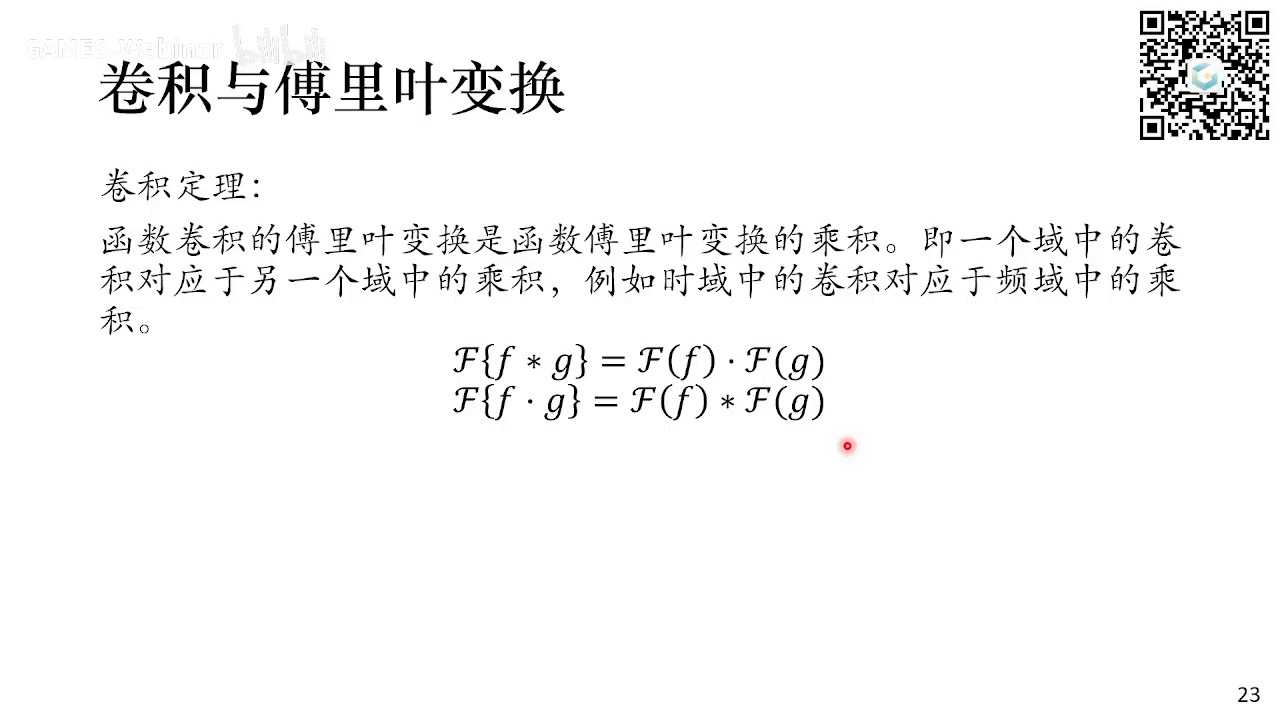
\includegraphics[width=0.92\textwidth]{figures/fig_22_conv_theorem.jpg}
\caption{卷积定理：一个域中的卷积对应另一个域中的乘积\vtag}
\end{figure}
\srcnote{00:44:45--00:45:00}
\end{minipage}


用这个定理重新看平均核：把 $3\times3$ 的平均核放到与图片同样大小的空间里做傅里叶变换，得到的频谱中心最亮，随着频率增高振幅衰减，图案很像小孔衍射的光斑。时域里用它卷积图片，等价于频域里把图片的频谱与这个频谱相乘：低频部分权重大，被保留；高频部分大多是黑的，权重很小，被抑制。这就是平均核让图片变平滑的原因，它本质上是一个低通滤波器。

\noindent\begin{minipage}{\textwidth}
\begin{figure}[H]
\centering
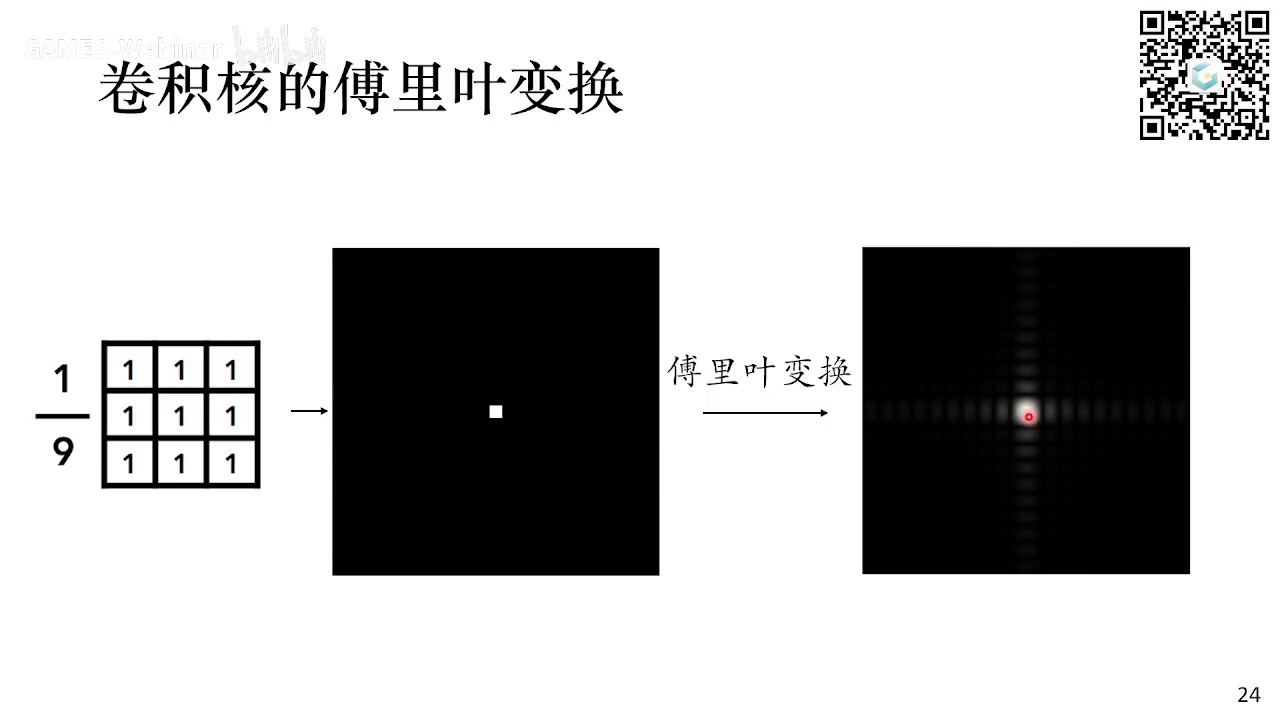
\includegraphics[width=0.92\textwidth]{figures/fig_23_kernel_ft.jpg}
\caption{平均核的傅里叶变换：中心亮、高频衰减\vtag}
\end{figure}
\srcnote{00:46:15--00:46:30}
\end{minipage}


\noindent\begin{minipage}{\textwidth}
\begin{figure}[H]
\centering
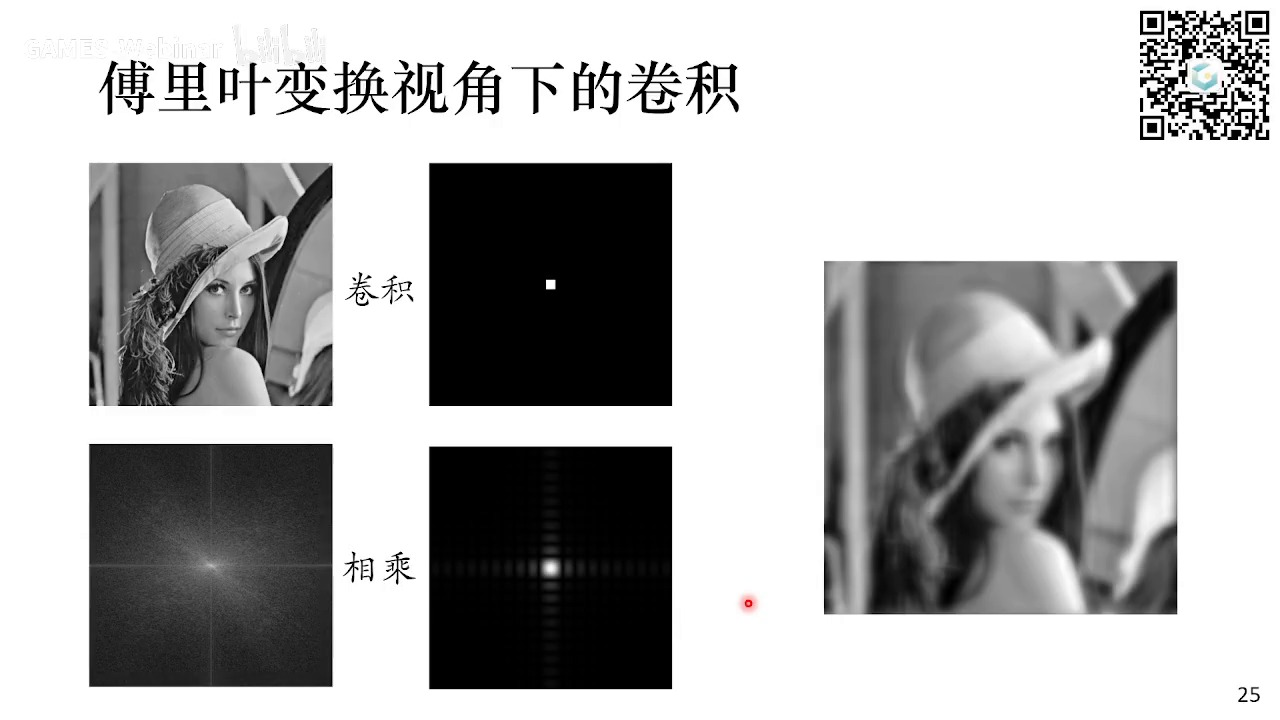
\includegraphics[width=0.92\textwidth]{figures/fig_24_conv_freq.jpg}
\caption{傅里叶变换视角下的卷积：时域卷积等价于频域相乘\vtag}
\end{figure}
\srcnote{00:47:45--00:48:00}
\end{minipage}


\begin{knowledgebox}{为什么用 FFT 算卷积}
讲义作者补充：直接计算长度为 $N$ 的信号与长度为 $M$ 的核的卷积需要 $O(NM)$ 次乘法；用卷积定理，先做 FFT、在频域逐点相乘、再做逆 FFT，总共只需 $O(N\log N)$。当核很大时（例如大半径的模糊、渲染中的大范围滤波），频域卷积会快得多。
\end{knowledgebox}

\section{采样与走样}

\subsection{采样是乘法}

现在用卷积定理分析采样。采样可以看成一个乘法过程：把连续函数 $f(t)$ 乘以梳状函数（Dirac comb）
\[
C_T(t)=\sum_{n=-\infty}^{\infty}\delta(t-nT),
\]
它是间隔为 $T$ 的一串 Delta 函数。$f(t)C_T(t)$ 只在 $t=nT$ 处有值，就是采样结果。

\noindent\begin{minipage}{\textwidth}
\begin{figure}[H]
\centering
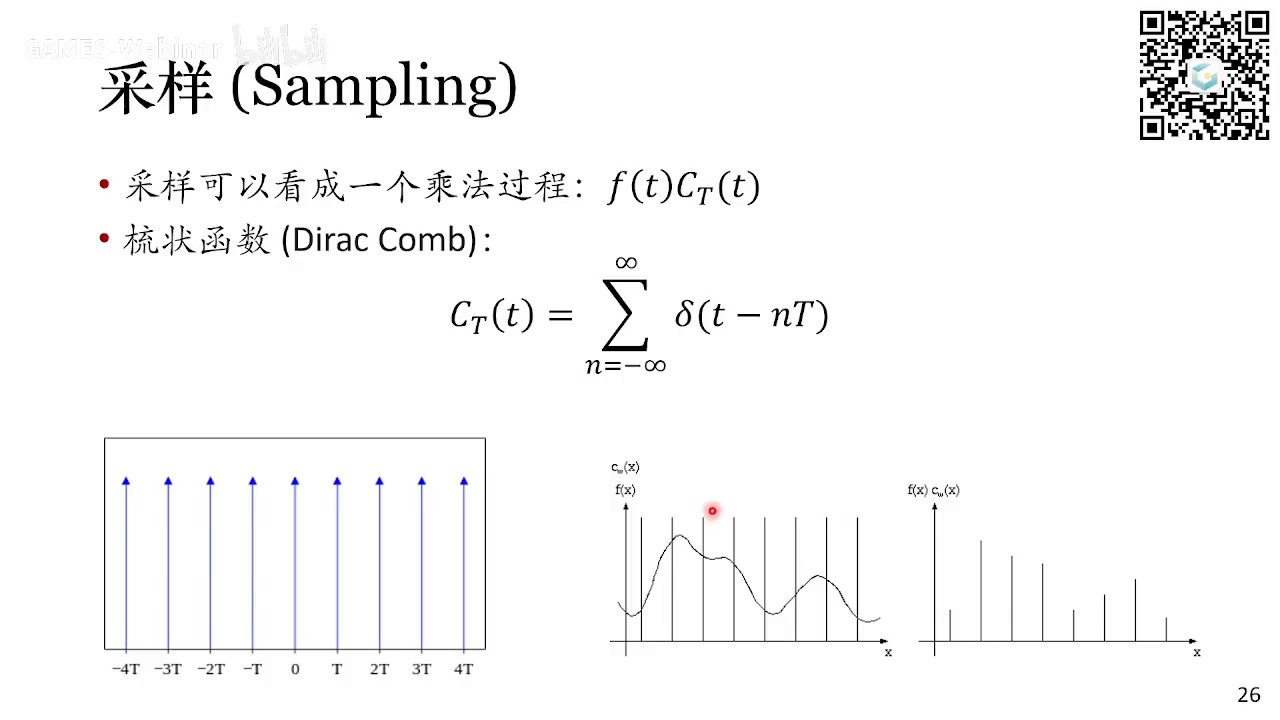
\includegraphics[width=0.92\textwidth]{figures/fig_25_sampling.jpg}
\caption{采样可以看成乘法：$f(t)C_T(t)$，梳状函数是一串等距的 Delta 函数\vtag}
\end{figure}
\srcnote{00:49:30--00:49:45}
\end{minipage}


\subsection{梳状函数的傅里叶变换}

要知道采样在频域对应什么，首先要求梳状函数的傅里叶变换。梳状函数是周期为 $T$ 的周期函数，可以先求傅里叶级数。在 $[-T/2,T/2)$ 内它只在零点处有值，利用 Delta 函数的性质：
\[
c_n=\frac1T\int_{-T/2}^{T/2}C_T(t)\,e^{-i\frac{2n\pi}{T}t}\,\mathrm dt=\frac1T,\qquad
C_T(t)=\sum_{n=-\infty}^{\infty}\frac1T\,e^{i\frac{2n\pi t}{T}} .
\]
也就是说，$C_T(t)$ 只有离散的频率分量，都是 $2\pi/T$ 的整数倍。

\noindent\begin{minipage}{\textwidth}
\begin{figure}[H]
\centering
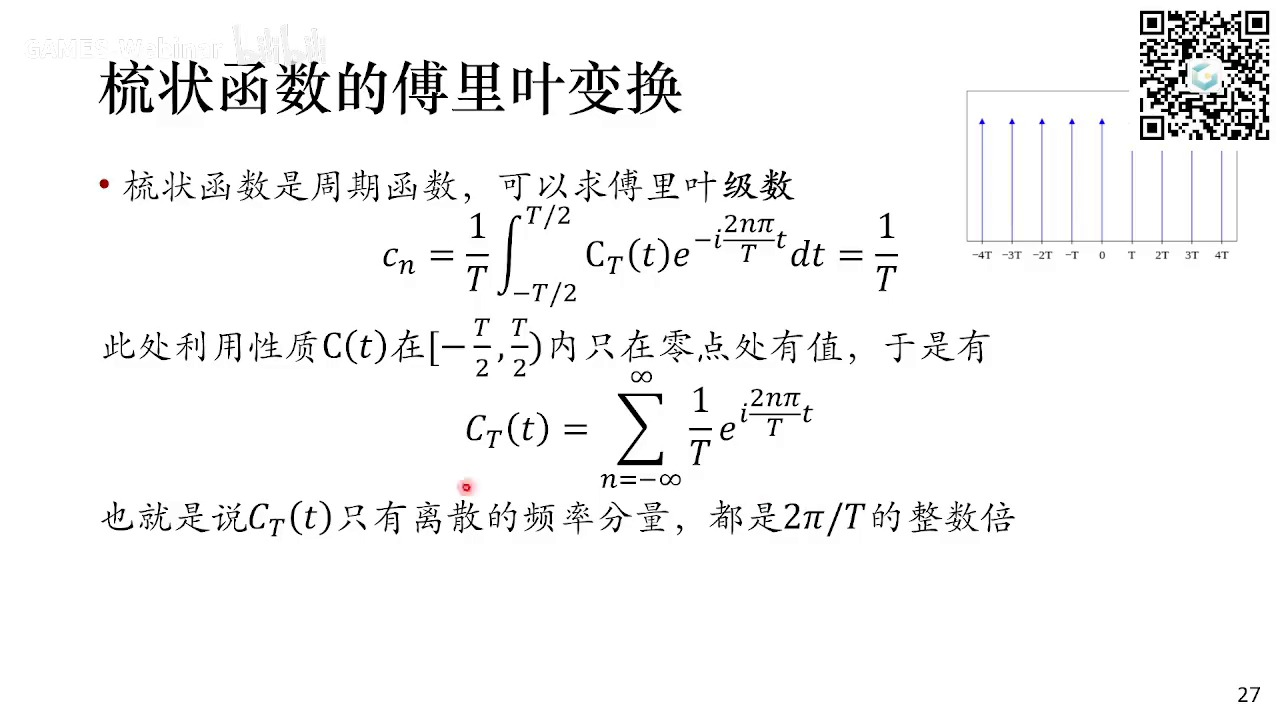
\includegraphics[width=0.92\textwidth]{figures/fig_26_comb_series.jpg}
\caption{梳状函数的傅里叶级数：系数都是 $1/T$，频率为 $2\pi/T$ 的整数倍\vtag}
\end{figure}
\srcnote{00:51:45--00:52:00}
\end{minipage}


对这种周期性的求和，可以再用梳状函数把它改写成积分：
\[
\sum_{n=-\infty}^{\infty}\frac1T\,e^{i\frac{2\pi n t}{T}}=\int_{-\infty}^{\infty}\frac1T\,C_{\frac{2\pi}{T}}(\omega)\,e^{i\omega t}\,\mathrm d\omega .
\]
注意这里导出的梳状函数周期是 $2\pi/T$。对比傅里叶变换的形式 $f(t)=\int F(\omega)e^{i\omega t}\mathrm d\omega$，就得到：周期为 $T$ 的梳状函数的傅里叶变换，是周期为 $2\pi/T$ 的梳状函数：
\[
\mathcal F\big(C_T(t)\big)=\frac1T\,C_{\frac{2\pi}{T}}(\omega).
\]
时域中采样越密（$T$ 越小），频域中梳齿的间隔 $2\pi/T$ 越大。

\noindent\begin{minipage}{\textwidth}
\begin{figure}[H]
\centering
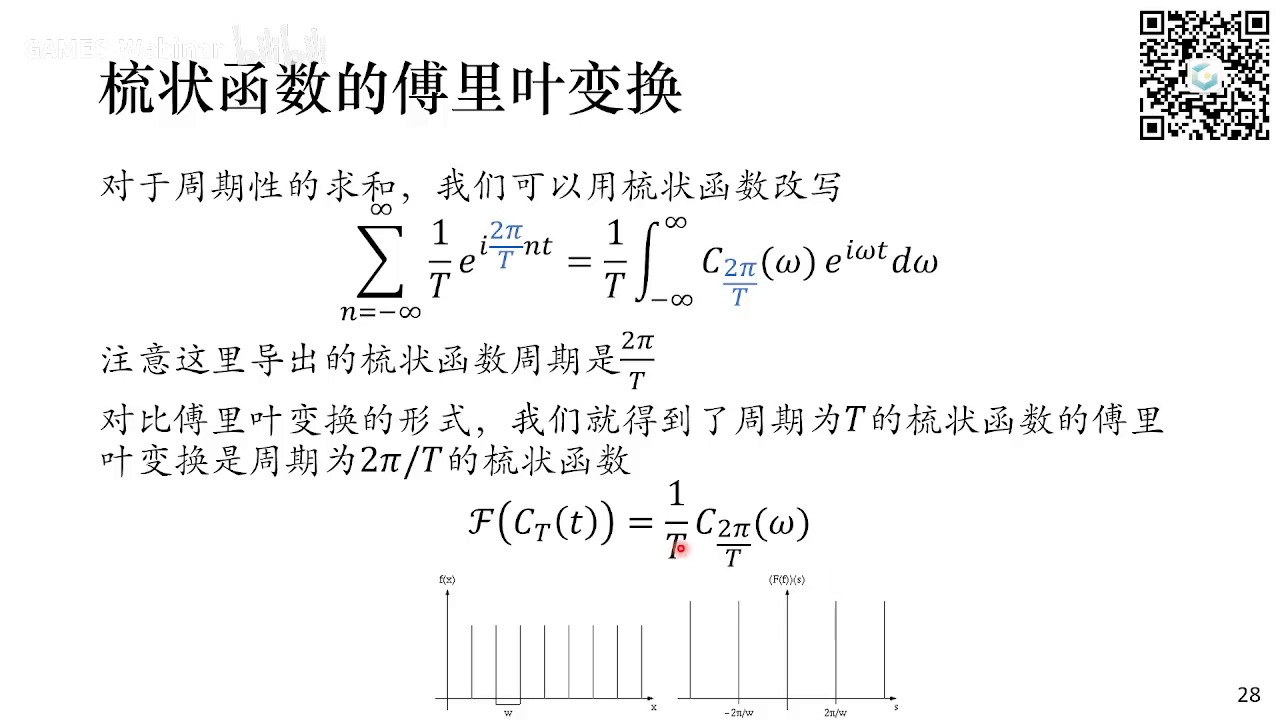
\includegraphics[width=0.92\textwidth]{figures/fig_27_comb_ft.jpg}
\caption{周期为 $T$ 的梳状函数的傅里叶变换是周期为 $2\pi/T$ 的梳状函数\vtag}
\end{figure}
\srcnote{00:54:00--00:54:15}
\end{minipage}


\subsection{采样在频域中是周期重复}

由卷积定理，时域的采样乘法对应频域的卷积。先看 $F(\omega)$ 与一个 Delta 函数的卷积：
\[
F(\omega)*\delta(\omega-\omega')=\int F(a)\,\delta(\omega-\omega'-a)\,\mathrm da=F(\omega-\omega'),
\]
结果是把 $F(\omega)$ 平移到 $\omega'$。梳状函数是一串 Delta 函数，所以 $F(\omega)$ 与 $C_{2\pi/T}(\omega)$ 卷积，就是把 $F(\omega)$ 每隔 $2\pi/T$ 平移复制一份，再叠加起来。$2\pi/T$ 正是采样频率（角频率）。这就是第三句话：时域上的采样等价于频域上的周期重复。

\noindent\begin{minipage}{\textwidth}
\begin{figure}[H]
\centering
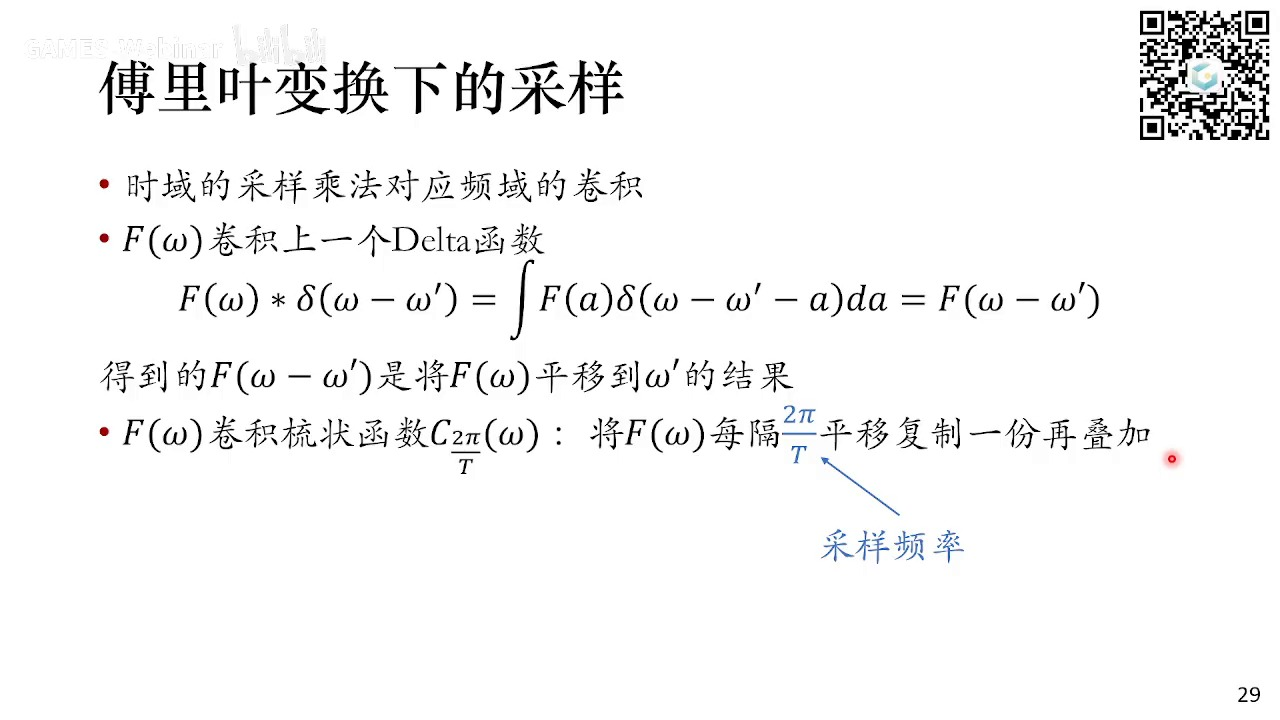
\includegraphics[width=0.92\textwidth]{figures/fig_28_sampling_freq.jpg}
\caption{傅里叶变换下的采样：频谱与梳状函数卷积，每隔 $2\pi/T$ 复制一份\vtag}
\end{figure}
\srcnote{00:57:00--00:57:15}
\end{minipage}


\noindent\begin{minipage}{\textwidth}
\begin{figure}[H]
\centering
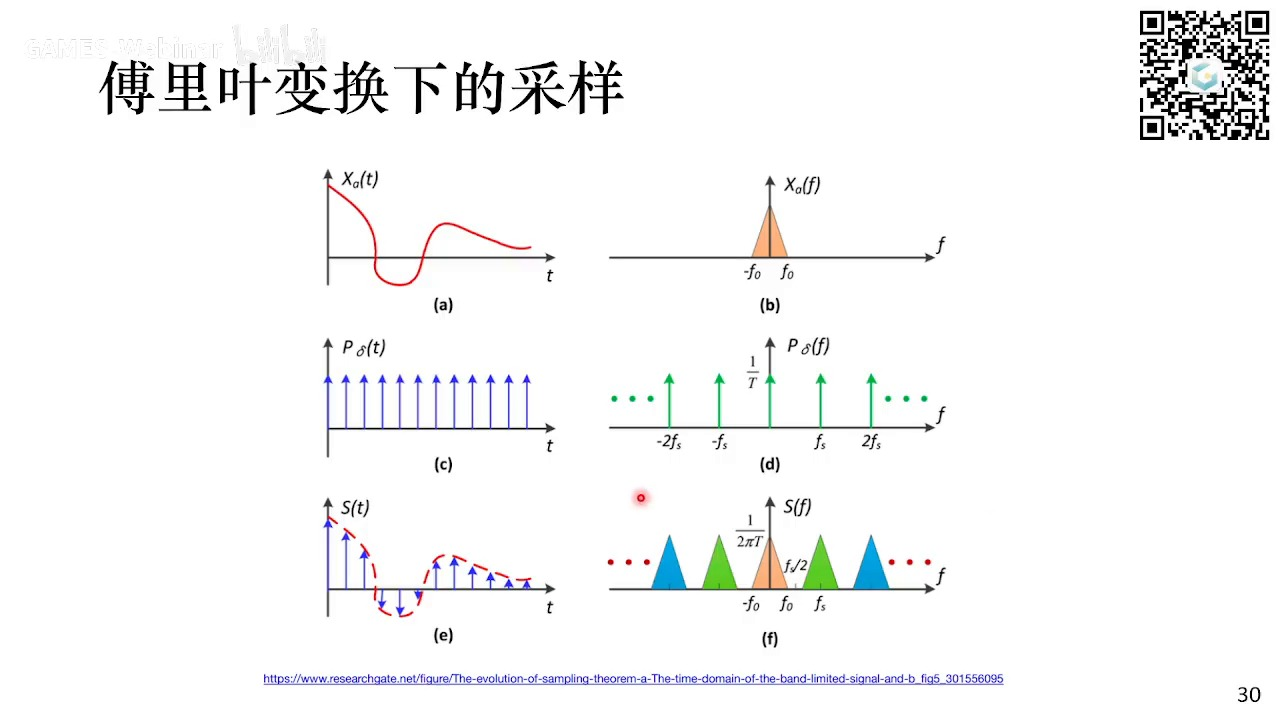
\includegraphics[width=0.92\textwidth]{figures/fig_29_sampling_process.jpg}
\caption{采样的完整过程：时域相乘、频域卷积，频谱被周期性复制\vtag}
\end{figure}
\srcnote{00:58:15--00:58:30}
\end{minipage}


\subsection{走样}

频谱被周期性复制以后，会发生什么取决于采样频率。如果采样足够密（dense sampling），频域中复制的间隔很大，各份频谱互不重叠，可以把中间那一份完整地取出来，从而恢复原函数。如果采样太稀疏（sparse sampling），复制的间隔太小，相邻的频谱会互相重叠，高频部分混入了低频部分，这就是\textbf{走样}（aliasing）。此时采到的东西已经不像原来的信号了，再也无法从采样结果恢复原函数。

\noindent\begin{minipage}{\textwidth}
\begin{figure}[H]
\centering
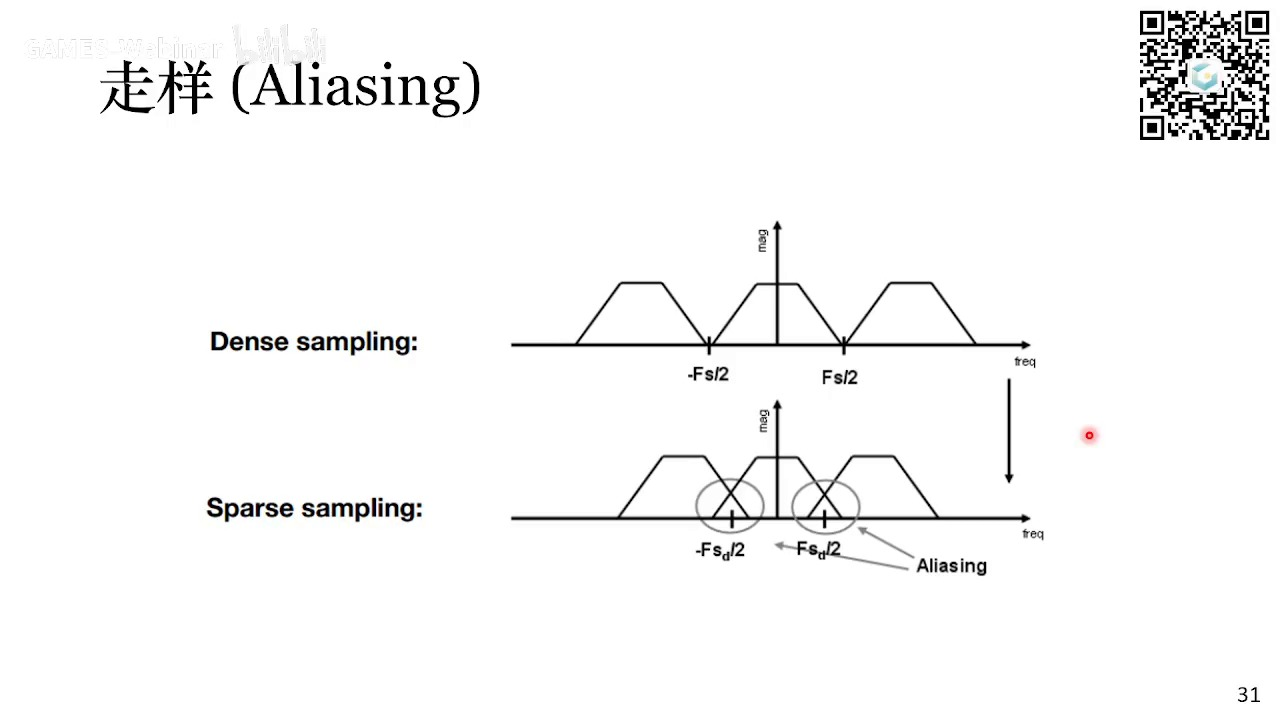
\includegraphics[width=0.92\textwidth]{figures/fig_30_aliasing.jpg}
\caption{走样：采样太稀疏时，复制的频谱相互重叠\vtag}
\end{figure}
\srcnote{01:00:00--01:00:15}
\end{minipage}


\begin{importantbox}{采样定理与反走样}
讲义作者补充：若原信号的最高角频率为 $\omega_{\max}$，频谱复制后不重叠的条件是 $2\pi/T>2\omega_{\max}$，即采样频率要高于信号最高频率的两倍，这就是奈奎斯特—香农采样定理。图形学中的反走样（anti-aliasing）正是从这里出发：要么提高采样率（超采样），要么在采样前先做低通滤波（模糊），把超出采样能力的高频去掉，使复制的频谱不再重叠。前面“卷积”与“采样”两部分合在一起，就解释了 GAMES101 中“先模糊后采样”的反走样方法为什么有效。
\end{importantbox}

\section{球谐函数}

\subsection{球坐标与渲染中的球面函数}

最后一部分是球谐函数。先回顾球坐标（spherical coordinate）：用两个角度 $\varphi\in[0,2\pi)$、$\theta\in[0,\pi]$ 和半径 $r$ 三个变量，同样能唯一确定空间中的任意点，其中 $r$ 标定从原点射出去多远。为什么要引入球坐标？因为渲染中有很多定义在球面上的函数 $f(\theta,\varphi)$，只与方向有关。例如环境球（environment map）记录了从各个方向射来的光照，球上每个点对应一个方向 $(\theta,\varphi)$；又如反射分布函数（BRDF）描述了光从一个方向入射后向各个方向反射的比例。

\noindent\begin{minipage}{\textwidth}
\begin{figure}[H]
\centering
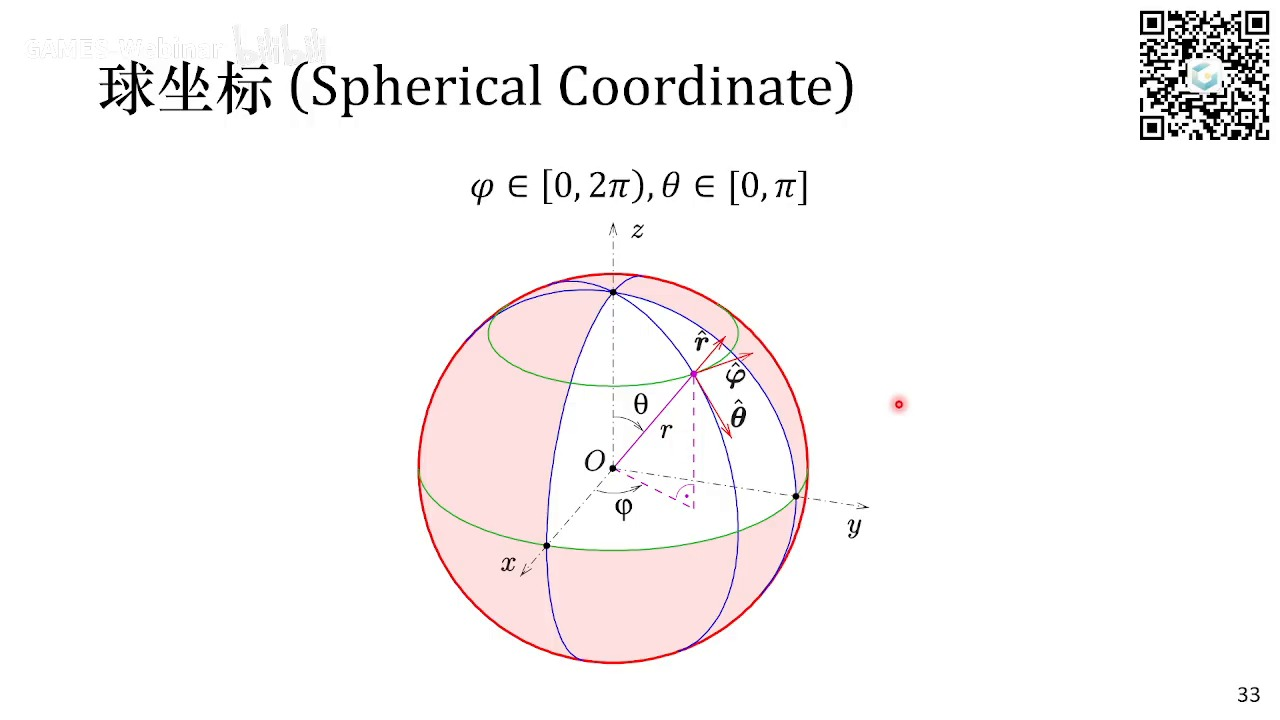
\includegraphics[width=0.92\textwidth]{figures/fig_31_spherical_coord.jpg}
\caption{球坐标：$\varphi\in[0,2\pi)$，$\theta\in[0,\pi]$\vtag}
\end{figure}
\srcnote{01:02:00--01:02:15}
\end{minipage}


\noindent\begin{minipage}{\textwidth}
\begin{figure}[H]
\centering
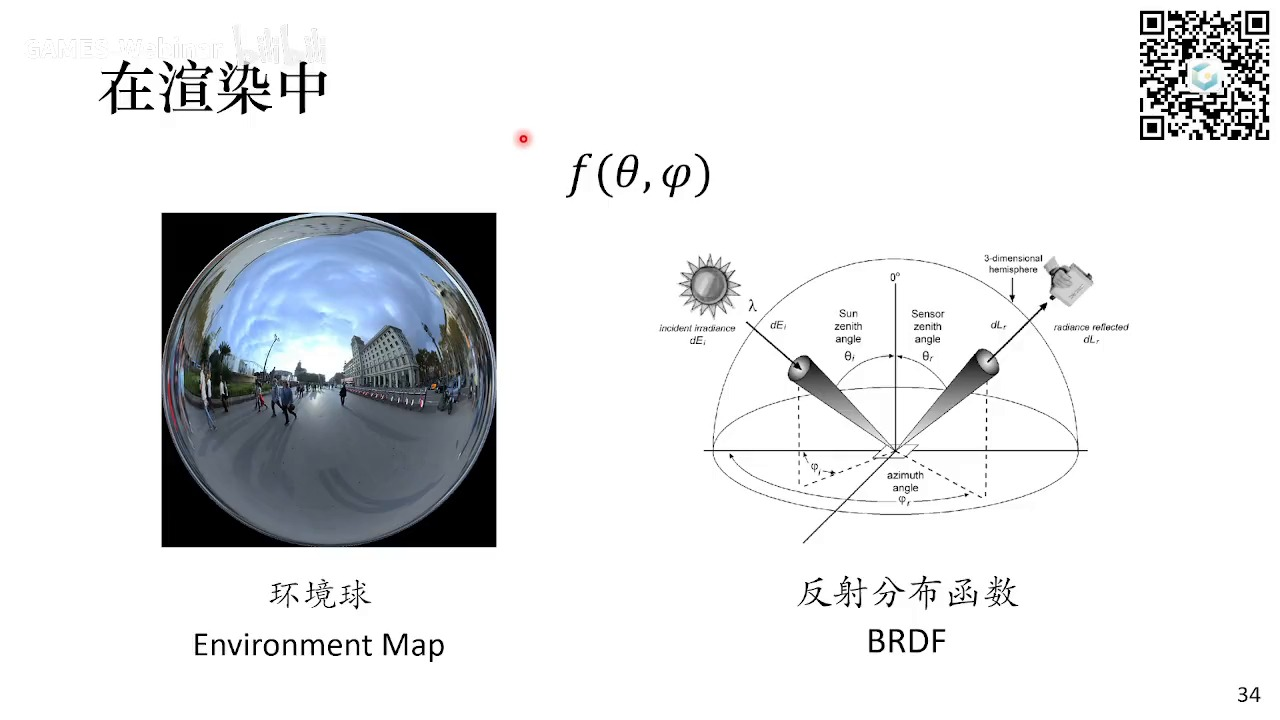
\includegraphics[width=0.92\textwidth]{figures/fig_32_rendering_sphere.jpg}
\caption{渲染中的球面函数：环境球与反射分布函数（BRDF）\vtag}
\end{figure}
\srcnote{01:03:45--01:04:00}
\end{minipage}


\subsection{球谐函数的定义}

球谐函数的表达式为
\[
Y_l^m(\theta,\varphi)=\sqrt{\frac{2l+1}{4\pi}\frac{(l-m)!}{(l+m)!}}\;P_l^m(\cos\theta)\;e^{im\varphi}.
\]
讲者说，可以不管里面的具体细节，把它分成三部分来看：第一部分是一个常数，$l$ 和 $m$ 是两个整数，$l\ge0$，$-l\le m\le l$；第二部分 $P_l^m(\cos\theta)$ 是 $\cos\theta$ 的伴随勒让德多项式，是关于 $\cos\theta$ 的多项式，阶数与 $l$ 有关；最后一部分 $e^{im\varphi}$ 是关于 $\varphi$ 的三角函数。

可视化时，沿 $(\theta,\varphi)$ 方向射出一条长度为 $|Y_l^m(\theta,\varphi)|$ 的射线，得到一个三维形状。课件把这些形状排成一个三角形阵列：从上到下 $l$ 增大，形状的“瓣”增多，对应频率增大；从左到右 $m$ 变化，瓣的分布方式不同，对应不同的“相位”，类似正弦与余弦的区别。

\noindent\begin{minipage}{\textwidth}
\begin{figure}[H]
\centering
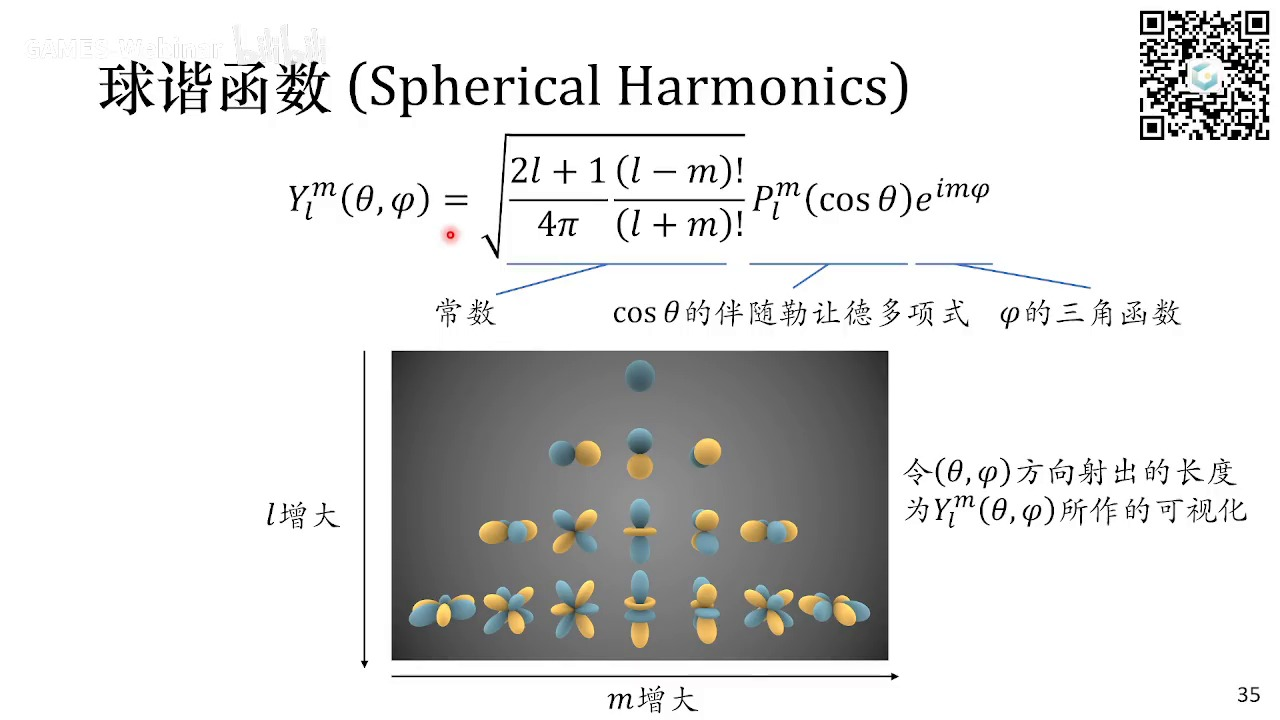
\includegraphics[width=0.92\textwidth]{figures/fig_33_sh_definition.jpg}
\caption{球谐函数的定义与可视化：$l$ 增大对应频率增大，$m$ 对应不同相位\vtag}
\end{figure}
\srcnote{01:07:00--01:07:15}
\end{minipage}


\noindent\begin{minipage}{\textwidth}
\begin{figure}[H]
\centering
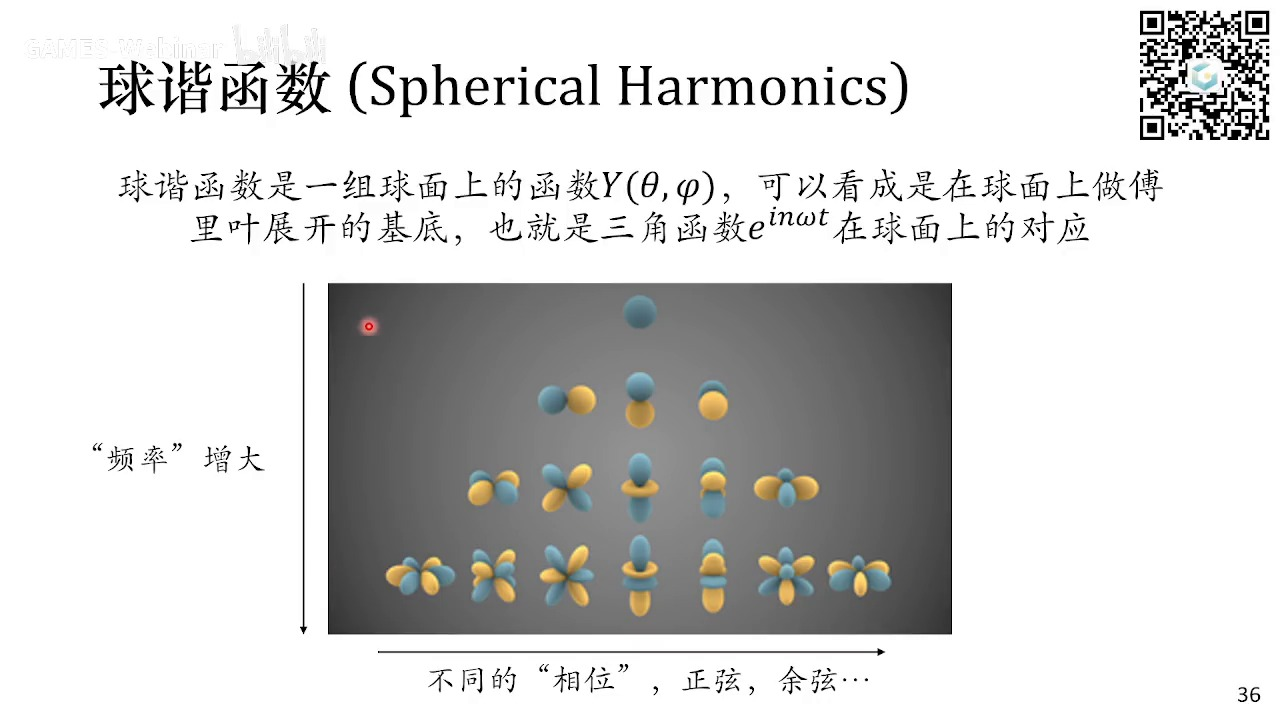
\includegraphics[width=0.92\textwidth]{figures/fig_34_sh_meaning.jpg}
\caption{球谐函数可以看成球面上做傅里叶展开的基底\vtag}
\end{figure}
\srcnote{01:08:00--01:08:15}
\end{minipage}


\subsection{球谐展开}

球谐函数是一组球面上的函数，可以看成是在球面上做傅里叶展开的基底，也就是三角函数 $e^{in\omega t}$ 在球面上的对应。任意球面函数都可以展开为
\[
f(\theta,\varphi)=\sum_{l=0}^{n}\sum_{m=-l}^{l}C_l^m\,Y_l^m(\theta,\varphi),\qquad
C_l^m=\int_0^{2\pi}\!\!\int_0^{\pi}f(\theta,\varphi)\,Y_l^m(\theta,\varphi)\sin\theta\,\mathrm d\theta\,\mathrm d\varphi .
\]
它可以一一对应到傅里叶级数：傅里叶级数用的是三角函数，这里用的是球谐函数；系数同样由函数与基函数的内积给出，$\sin\theta$ 是球面上的面积元。展开到 $l\le n$，就相当于只保留到某个频率上限的傅里叶级数。课件用不同截断阶数展开同一个球面函数：沿每个方向射出长度为 $f(\theta,\varphi)$ 的射线，阶数越高，形状越接近原函数。

\noindent\begin{minipage}{\textwidth}
\begin{figure}[H]
\centering
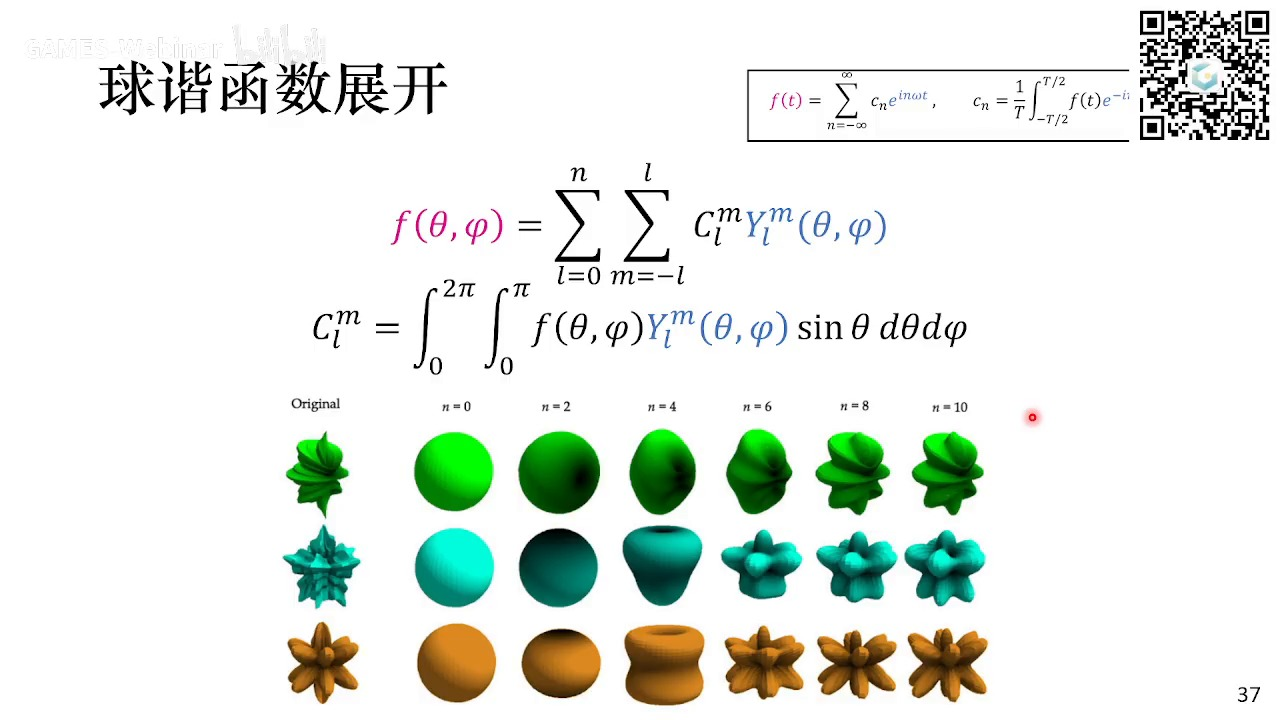
\includegraphics[width=0.92\textwidth]{figures/fig_35_sh_expansion.jpg}
\caption{球谐函数展开：系数为函数与基函数在球面上的内积\vtag}
\end{figure}
\srcnote{01:11:15--01:11:30}
\end{minipage}


\begin{warningbox}{实球谐与复球谐}
讲义作者补充：课件中的 $Y_l^m$ 含 $e^{im\varphi}$，是复值的；严格来说系数公式中应取共轭 $\overline{Y_l^m}$。渲染中常用的是实球谐函数，用 $\cos(m\varphi)$ 和 $\sin(|m|\varphi)$ 代替 $e^{im\varphi}$，这时不需要共轭。展开到 $l\le n$ 共有 $(n+1)^2$ 个系数，例如 3 阶（$l\le2$）共 9 个，这就是许多实时渲染引擎用 9 个系数存储环境漫反射光照的原因。
\end{warningbox}

\subsection{环境球压缩}

球谐函数的典型应用是环境球压缩：只保留低阶球谐展开中的权重 $C_l^m$，就能用很少的数据近似表达整个环境光照。用低阶球谐函数表示，会得到非常光滑的结果；它大体上符合原来环境球的分布，但细节被平滑掉了。这与图像的低通滤波完全是同一个道理，因为低阶球谐函数就是球面上的“低频”。对漫反射光照这种本身就很光滑的量，低阶近似已经足够。

\noindent\begin{minipage}{\textwidth}
\begin{figure}[H]
\centering
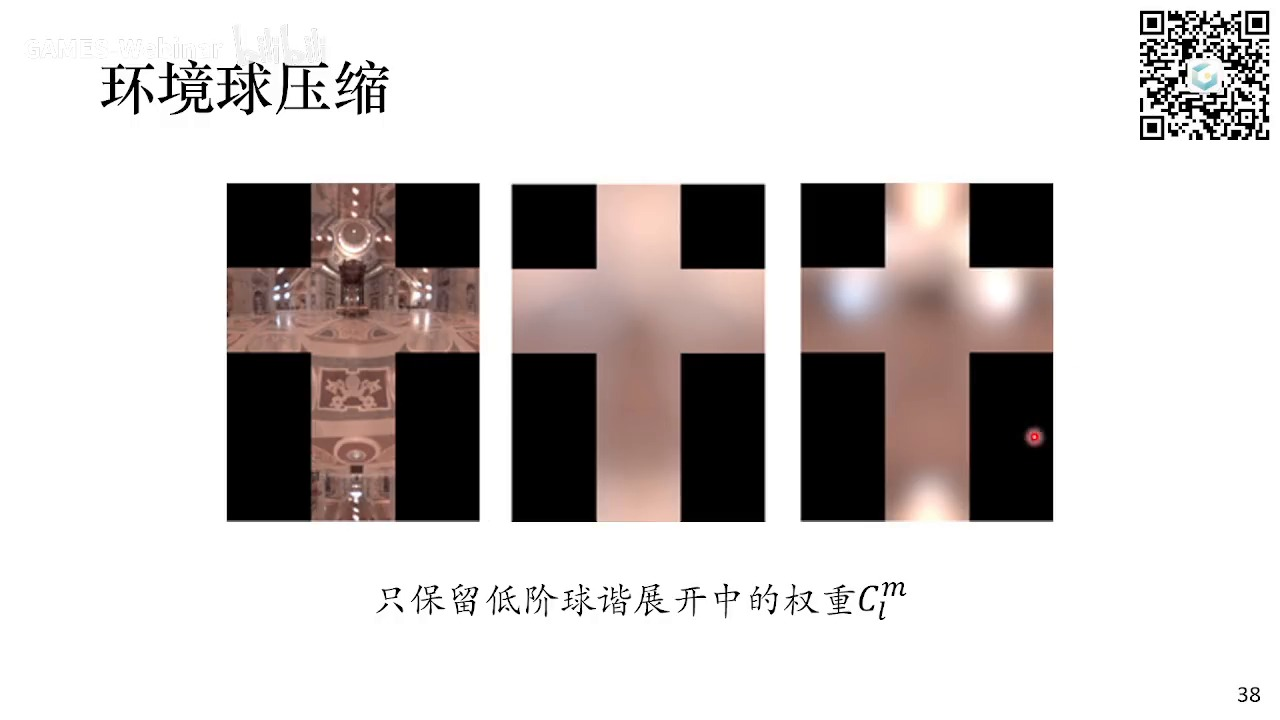
\includegraphics[width=0.92\textwidth]{figures/fig_36_env_compress.jpg}
\caption{环境球压缩：只保留低阶球谐展开的权重，得到光滑的近似\vtag}
\end{figure}
\srcnote{01:12:30--01:12:45}
\end{minipage}


\subsection{与傅里叶展开的联系}

为什么说球谐函数是“球面上的傅里叶基”？讲者给出了一个更深的联系，有兴趣的同学可以进一步研究。三维空间中的拉普拉斯算子为
\[
\nabla^2f=\frac{\partial^2f}{\partial x^2}+\frac{\partial^2f}{\partial y^2}+\frac{\partial^2f}{\partial z^2}.
\]
一维傅里叶展开的基函数 $e^{i\omega x}$ 是一维拉普拉斯算子的特征向量：
\[
\frac{\mathrm d^2}{\mathrm dx^2}e^{i\omega x}=-\omega^2e^{i\omega x},
\]
这正是 $\mathrm A\mathbf x=\lambda\mathbf x$ 的形式，$-\omega^2$ 就是特征值。而球谐函数正是球坐标下拉普拉斯算子角度部分的特征向量。球坐标下的拉普拉斯算子为
\[
\nabla^2f=\frac1{r^2}\frac{\partial}{\partial r}\Big(r^2\frac{\partial f}{\partial r}\Big)+\frac{1}{r^2\sin\theta}\frac{\partial}{\partial\theta}\Big(\sin\theta\frac{\partial f}{\partial\theta}\Big)+\frac{1}{r^2\sin^2\theta}\frac{\partial^2f}{\partial\varphi^2},
\]
在单位球面上只保留后两项，$Y_l^m$ 满足其特征方程，特征值为 $-l(l+1)$。所以“频率”在一维中由 $\omega$ 刻画，在球面上由 $l$ 刻画。

\noindent\begin{minipage}{\textwidth}
\begin{figure}[H]
\centering
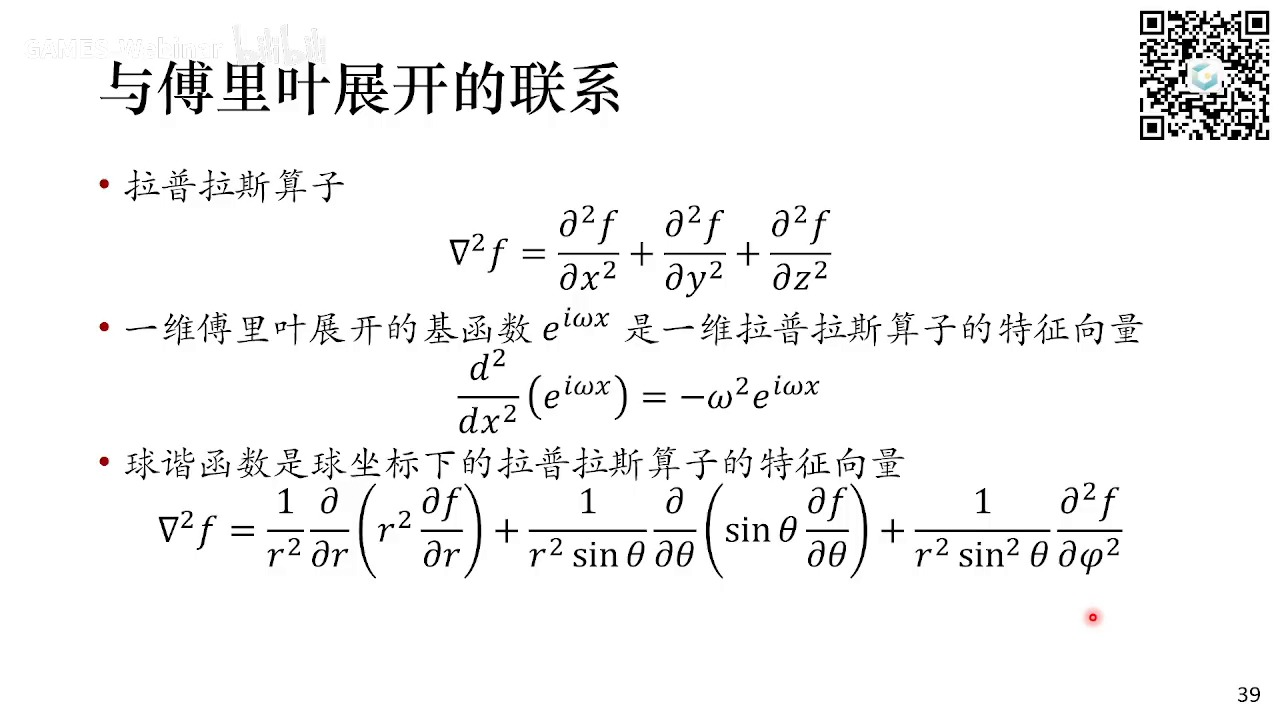
\includegraphics[width=0.92\textwidth]{figures/fig_37_laplacian.jpg}
\caption{与傅里叶展开的联系：二者都是拉普拉斯算子的特征函数\vtag}
\end{figure}
\srcnote{01:15:00--01:15:15}
\end{minipage}


\section{总结}

讲者最后重申了本讲的四个核心观点：傅里叶变换是从时域基底换到频域基底的线性变换；时域上的相乘等价于频域上的卷积，反之亦然；时域上的采样等价于频域上的周期重复；球谐函数是傅里叶展开在球坐标下的基底。课后有同学问到渲染中更具体的球谐应用，讲者表示那部分属于渲染课程的知识，就不在这里展开了。

\noindent\begin{minipage}{\textwidth}
\begin{figure}[H]
\centering
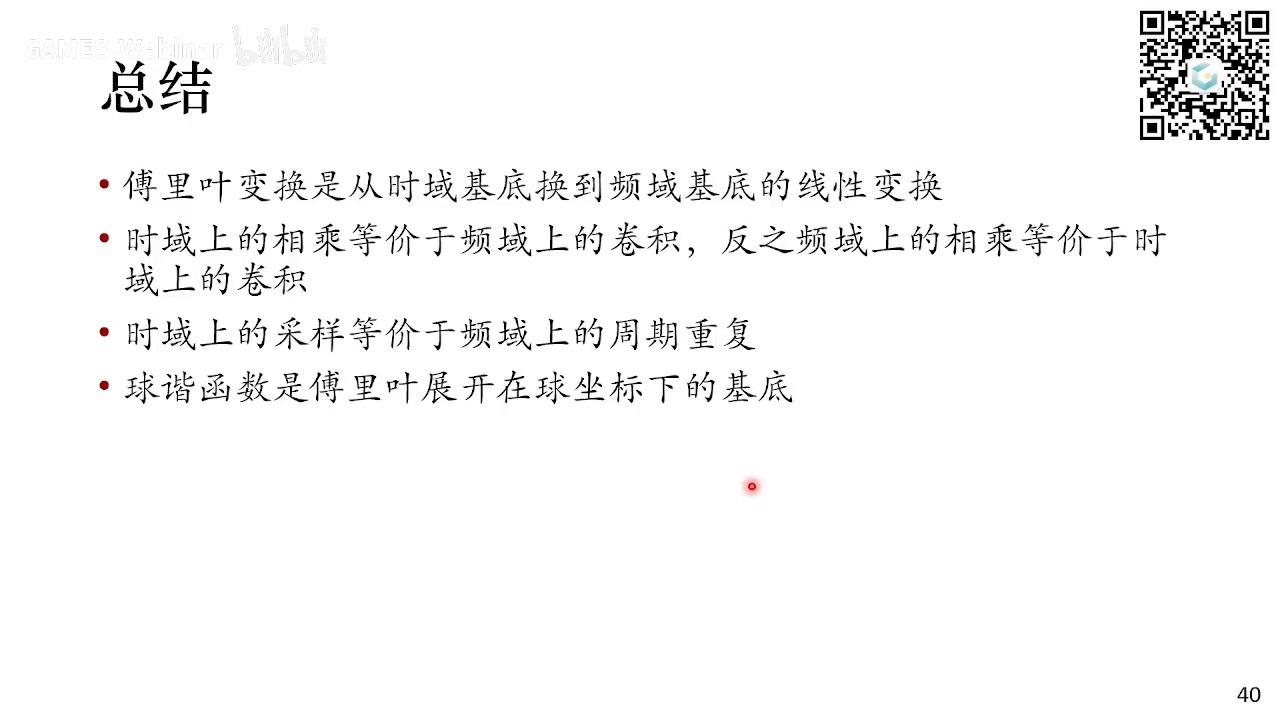
\includegraphics[width=0.92\textwidth]{figures/fig_38_summary.jpg}
\caption{总结：傅里叶变换、卷积定理、采样与球谐函数\vtag}
\end{figure}
\srcnote{01:18:00--01:18:15}
\end{minipage}


\begin{practicebox}{自测清单}
\begin{itemize}
\item 写出方波的傅里叶展开，说明频谱为什么只含奇数倍频率、振幅为什么递减。
\item 从傅里叶级数的指数形式取 $T\to\infty$ 的极限，得到傅里叶变换对。
\item 用 Delta 函数的积分恒等式解释“写出 $f(t)$ 就是在 Delta 基下给出系数”。
\item 用卷积定理解释平均核为什么是低通滤波器。
\item 推导梳状函数的傅里叶变换，并说明采样频率与频域复制间隔的关系。
\item 说明走样的成因，以及“先模糊后采样”为什么能反走样。
\item 数一数球谐展开到 $l\le n$ 时的系数个数，并解释环境球压缩为什么得到光滑结果。
\end{itemize}
\end{practicebox}

\end{document}
